\documentclass[twoside,twocolumn]{mnras}

% Paper packages
\usepackage{graphicx}
\usepackage{amsmath}
\usepackage{amssymb}
\usepackage{natbib}

% Define astronomical units
\newcommand{\msun}{\ensuremath{M_{\odot}}}
\newcommand{\pc}{\ensuremath{\rm pc}}
\newcommand{\kms}{\ensuremath{\rm km\,s^{-1}}}

\title{Fragmentation of Interstellar Filaments: Complete HGBS Analysis and MHD Simulations}

\author[G.~J.~White]{G.~J.~White$^{1,2}$\\
$^{1}$School of Physical Sciences, The Open University, Walton Hall, Milton Keynes, MK7 6AA, UK\\
$^{2}$Rutherford Appleton Laboratory, Harwell Science and Innovation Campus, Didcot, OX11 0QX, UK}

\begin{document}

\maketitle

\begin{abstract}
Classical fragmentation theory predicts core spacing ${\sim}4\times$ the filament
width, yet Herschel measures $\lambda/W \approx 2$--$3$. We reanalyse core spacing
in Herschel Gould Belt Survey (HGBS) filaments using Gaia DR3 distances and 2,013
self-gravitating MHD simulations. Four robust regions give $\lambda/W = 2.84$
($0.284 \pm 0.026$~pc); the full 8-region sample (5,069 cores) gives $2.79 \pm 0.025$~pc
(jackknife; bootstrap $\pm 0.009$~pc). \textit{All measurements use the pairwise median
statistic; nearest-neighbour statistics are available only for Taurus. The L/3 convergence
bias of unknown magnitude is the dominant methodological caveat.} Excluding the two
highest-revision regions (Aquila $+68\%$; Orion~B $+48\%$) reduces the mean to
$0.231$~pc ($-17\%$), confirming sensitivity to these independently verified distances.
After 3D projection correction the inferred spacing is ${\sim}3.5\times W$, within 15\%
of the classical prediction \citep{Inutsuka1992}.

Magnetic tension for longitudinal fields ($\beta = 1$--$3$) predicts
$\lambda/W = 2.44$--$3.16$ but requires longitudinal geometry (${\sim}10\%$ of dense
filaments; \citealt{Planck2016}); perpendicular-field simulations give
$\lambda/W \approx 1.25$---a factor ${\sim}2.2\times$ below observations (Section~\ref{sec:perp_paradox}).
Hierarchical fibre fragmentation is the more observationally consistent interpretation.

Simulations reveal $1/t_{\rm frag} \propto f^{0.39}$ ($r^2 = 0.999$). Supercritical
filaments ($f \geq 1.5$) undergo radial collapse; \textit{the simulations cannot
directly measure $\lambda/W$ in this regime}---all comparisons rest on near-critical
calibration ($f = 0.9$--$1.3$). Near-critical filaments ($f \lesssim 1.2$) produce
longitudinal beading. The Plummer width correction ($T1 = 0.707 \pm 0.04$) places
low-$\beta$ configurations at or exceeding the HGBS window boundary; the magnetic
tension scenario cannot be assessed within current simulation uncertainties.
\end{abstract}

\begin{keywords}
stars: formation -- ISM: structure -- ISM: filaments -- MHD -- turbulence
\end{keywords}

\section{INTRODUCTION}

The \textit{Herschel} Space Observatory established that filaments are the fundamental
structures within which star formation occurs in molecular clouds \citep{Andre2010}.
Two key observational results emerged: (1) a characteristic filament width of $\sim$0.1~pc
across diverse environments \citep{Arzoumanian2011}, and (2) a critical mass-per-unit-length
of $M_{\rm line,crit} \approx 16~M_\odot$/pc \citep{Ostriker1964}.

Classical fragmentation theory \citep{Inutsuka1992} predicts that isothermal gas cylinders
fragment at a wavelength of approximately $4\times$ the filament width. For the
characteristic HGBS width of $0.10$~pc, this predicts a core spacing of $\sim 0.4$~pc.
Original HGBS analyses measured spacings of $\sim 0.2$~pc---nearly a factor of two below
this prediction. With Gaia DR3 distances \citep{Zhang2023}, measured spacings have
increased to $\sim 0.28$~pc, reducing the discrepancy to a factor of 1.4.

Two primary explanations have been proposed. First, \textbf{hierarchical fragmentation}:
high-resolution studies show that filaments consist of velocity-coherent fibres
\citep{Hacar2013}, and recent work in Orion~B \citep{Yang2024} shows that fibre-to-core
spacing recovers the classical $4\times$ prediction while filament-to-core measurements
show sub-Jeans values. Second, \textbf{magnetic tension}: longitudinal fields shift the
most unstable mode to shorter wavelengths \citep{Nakamura1993}, predicting
$\lambda/W \approx 2.44$--$3.16$ for equipartition fields ($\beta \sim 1$--$3$).

Here we present a systematic analysis of all 8 high-confidence HGBS regions using Gaia DR3 distances and a uniform pairwise-median methodology, combined with 2,013 self-gravitating MHD simulations. Observationally, hierarchical fibre fragmentation is the most consistent interpretation (based on single-region evidence from \citealt{Yang2024}); the simulations presented here constrain single-component MHD fragmentation and do not directly test hierarchical structure. Magnetic tension in a strictly longitudinal, low-$\beta$ ($\beta \leq 0.5$) geometry is a secondary possibility, but whether it is viable within simulation uncertainties depends on the T1 width correction (T1$=0.606$--$0.707$; Section~\ref{sec:width_correction}).

\section{OBSERVATIONAL ANALYSIS}

\subsection{Complete HGBS Sample}
\label{sec:sample}

Our sample includes 8 high-confidence HGBS regions (Table~\ref{tab:sample}), with
distances updated to Gaia DR3-based measurements from \citet{Zhang2023}.

\textbf{Distance revisions}: The most significantly affected regions are Serpens
($260 \to 458$~pc, $+76\%$), Aquila ($260 \to 436$~pc, $+68\%$), and Orion~B
($260 \to 386$~pc, $+48\%$). Taurus shows a small decrease ($140 \to 135$~pc, $-4\%$).

\textbf{Core selection}: We include starless, prestellar, and protostellar cores following the standard HGBS framework \citep{Konyves2015, Konyves2020}. As a cross-check, using only the 331 Taurus starless cores gives $\lambda/W = 2.03$---within 2.5\% of the all-core value---confirming that protostellar inclusion does not bias the result.

\begin{table*}
\caption{Complete HGBS Sample with Gaia DR3 Distances}
\label{tab:sample}
\begin{tabular}{lcccccc}
\toprule
Region & Distance & Total & Spacing & Std Error & Beam (pc) & Status \\
       & (pc)   & Cores & (pc)   & (pc)      & (pc) & \\
\midrule
Orion B  & 386 & 1,844 & 0.313 & 0.047 & 0.034 & Robust \\
Aquila   & 436 & 749   & 0.346 & 0.047 & 0.038 & Robust \\
Perseus  & 296 & 816   & 0.248 & 0.040 & 0.026 & Robust \\
Taurus   & 135 & 536   & 0.198 & 0.040 & 0.012 & Robust \\
Ophiuchus& 137 & 513   & 0.206 & 0.053 & 0.012 & Limited \\
Serpens  & 458 & 194   & 0.331 & 0.097 & 0.040 & Limited \\
TMC1     & 135 & 178   & 0.195 & 0.056 & 0.012 & Limited \\
CRA      & 150 & 239   & 0.248 & 0.072 & 0.013 & Limited \\
\midrule
\textbf{Weighted Mean} &  & \textbf{5,069} & \textbf{0.279} & \textbf{0.009} & --- &  \\
\bottomrule
\end{tabular}
\\ \footnotesize \textbf{Note}: Beam scale = 18$''$ FWHM. Ophiuchus is classified as Limited (not Robust) despite $N>500$ because of larger distance uncertainty and slightly lower completeness.
\end{table*}

\subsection{Measurement Methodology}

Filament skeletons were identified using DisPerSE \citep{Sousbie2011} following standard
HGBS methodology with a $3\sigma$ persistence threshold and a robustness/filament-contrast
threshold of $\kappa = 2.0$ (standard HGBS parameters; \citealt{Arzoumanian2011}). Gaia DR3 distance revisions
do not require re-extraction of skeletons; physical scales are updated by rescaling
angular positions. Core-to-core spacings were measured using the pairwise median
statistic: for a filament with $N$ cores, we compute all $N(N-1)/2$ pairwise distances
and take the median. Cores were associated with filaments using a perpendicular
distance threshold of $2\times$ the characteristic filament width; results change
by $<3\%$ across threshold choices of $1$--$2\times W$.

\subsection{Results}
\label{sec:results}

\textbf{Width systematic}: A $\sim$30\% systematic uncertainty from filament width
scatter ($0.05$--$0.20$~pc; \citealt{Panopoulou2022}) affects all $\lambda/W$ values
and is not included in bootstrap error bars; it dominates when comparing with theory.

\textbf{Primary result}: Four robust regions (Orion~B, Aquila, Perseus, Taurus;
$N > 500$) give $0.284 \pm 0.026$~pc jackknife ($\lambda/W = 2.84$; bootstrap
$\pm 0.012$~pc); the full 8-region sample gives $0.279 \pm 0.025$~pc jackknife
($\lambda/W = 2.79$; bootstrap $\pm 0.009$~pc). Jackknife errors are adopted as
primary throughout (Section~\ref{sec:statistics}); bootstrap CI given for reference.
Gaia DR3 raised the mean 32\% from $0.211$~pc; leave-one-out analysis
(Table~\ref{tab:leave_one_out}) shows no single region dominates ($\Delta < 6\%$);
leave-two-out (Aquila+Orion~B excluded) gives $0.231$~pc ($\lambda/W = 2.31$,
$\Delta = -16.8\%$; Table~\ref{tab:leave_one_out}).

Figure~\ref{fig:spacing} shows the spacing measurements. After the standard 3D projection
correction, we adopt $4/\pi \approx 1.27$ \citep{Andre2010}, corresponding to the
\citet{Hacar2013} finite-aspect-ratio value for filaments with aspect ratios ${\sim}10{:}1$
(range 1.18--1.41 for $5{:}1$--$20{:}1$; we adopt the fiducial $10{:}1$ value, systematic
uncertainty $\lesssim 10\%$). The inferred spacing is ${\sim}3.5\times W$, within 15\%
of the classical $4\times$ prediction.

Planck Collaboration (2016) found that the mean magnetic field is preferentially
perpendicular to dense filaments, which implies---under the additional assumption of
random filament orientations within the plane of sky---that such filaments lie
preferentially close to the plane of sky \citep{Planck2016}. This would reduce the
projection factor to ${\sim}1.10$--$1.20$, giving a corrected spacing of
${\sim}3.1$--$3.3\times W$---\textit{strengthening} rather than removing the residual
discrepancy with the $4\times$ prediction. We adopt the standard $4/\pi$ correction
to facilitate comparison with the existing HGBS literature, with $\lesssim10\%$
systematic uncertainty; the Planck-informed value would yield a larger residual discrepancy.

\begin{table}[h]
\caption{Leave-One-Out Sensitivity Analysis}
\label{tab:leave_one_out}
\begin{tabular}{lcccc}
\toprule
Excluded Region & Excl.\ spacing (pc) & Remaining mean (pc) & $\lambda/W$ & $\Delta$ (\%) \\
\midrule
None (full sample) & --- & 0.279 & 2.79 & 0.0 \\
Orion B & $0.313 \pm 0.047$ & 0.268 & 2.68 & $-3.9$ \\
Aquila & $0.346 \pm 0.047$ & 0.266 & 2.66 & $-4.7$ \\
Perseus & $0.248 \pm 0.040$ & 0.281 & 2.81 & $+0.7$ \\
Taurus & $0.198 \pm 0.040$ & 0.287 & 2.87 & $+2.9$ \\
Ophiuchus & $0.206 \pm 0.053$ & 0.286 & 2.86 & $+2.5$ \\
Serpens & $0.331 \pm 0.097$ & 0.276 & 2.76 & $-1.1$ \\
TMC1 & $0.195 \pm 0.056$ & 0.281 & 2.81 & $+0.7$ \\
CRA & $0.248 \pm 0.072$ & 0.279 & 2.79 & $0.0$ \\
\midrule
Robust only & --- & 0.284 & 2.84 & $+1.8$ \\
\textbf{Aquila $+$ Orion~B excl.} & --- & \textbf{0.231} & \textbf{2.31} & $\mathbf{-16.8}$ \\
\bottomrule
\end{tabular}
\vspace{2pt}
\footnotesize Bootstrap 95\% CI $[0.261, 0.298]$~pc; jackknife $1\sigma$: full sample $\pm 0.025$~pc; robust $\pm 0.026$~pc. With $N=8$ regions the bootstrap spans only $2^8=256$ distinct resamples, making the jackknife more reliable at this sample size. Excluding the two highest-revision regions (Aquila $+68\%$, Orion~B $+48\%$) reduces the mean by $16.8\%$; their Gaia distances are independently confirmed \citep{Yan2022,Green2024,Kounkel2018}, so this sensitivity reflects the real importance of accurate distances rather than systematic bias.
\end{table}

\subsection{Distance Uncertainties and Sample Heterogeneity}
\label{sec:distance_uncertainties}

We classify regions as \textbf{Robust} (Orion~B, Aquila, Perseus, Taurus: $N>500$,
well-established Gaia distances, $<15\%$ or validated revision) or \textbf{Limited}
(Ophiuchus, Serpens, TMC1, CRA (Corona Australis): smaller YSO samples and/or $>50\%$ revision).

\textbf{Serpens}: The +76\% distance revision ($260 \to 458$~pc) raises concern, but is independently confirmed at $440$--$460$~pc \citep{Yan2022, Green2024, Zucker2020}. Excluding Serpens changes the full-sample result by only 1.1\% (Table~\ref{tab:leave_one_out}).

\textbf{Serpens beam/completeness}: The $0.040$~pc beam (40\% of $W_{\rm fil}$) may
overestimate spacing by ${\sim}8\%$; at 3.8\% sample weight, impact on the mean is
$<0.2\%$. Serpens is classified as Limited.

\textbf{Aquila anomaly}: Aquila has the largest Robust spacing ($\lambda/W = 3.46$),
possibly from W40 H\,{\sc ii} feedback \citep{Bontemps2010} or the $+68\%$ distance
revision. The 436~pc distance is confirmed by 3D dust mapping \citep{Zucker2020} and
Gaia-parallax YSOs at $430 \pm 20$~pc \citep{Konyves2020}. We retain it as Robust,
noting exclusion reduces the robust mean by 6\%.

\textbf{Aquila protostellar cross-check}: The pairwise median is insensitive to
removal of $\sim$11.5\% of cores (protostellar fraction from \citealt{Konyves2015});
Monte Carlo resampling retaining 663 non-protostellar sources gives
$\lambda/W = 3.40 \pm 0.07$ vs.\ all-core value 3.46 ($<2\%$ change). \textit{This
demonstrates pairwise-median robustness to core-type contamination, not absence of
protostellar migration effects}; the two statements should not be conflated.
The Aquila elevated spacing remains an unresolved environmental outlier (W40 feedback;
$+68\%$ distance revision).

\textbf{Distance-spacing regression}: As expected, $\lambda \propto d$ ($r^2 = 0.91$;
the relationship is geometric, not evidence for physical uniformity). The residuals
test ($r = 0.18$, $p = 0.68$) demonstrates no obvious systematic bias in the
distance revisions, but with $N = 8$ regions this test has low statistical power
(type~II error rate ${\sim}60\%$) and cannot provide strong evidence against
systematic bias.

\subsection{Statistical Methods: Pairwise Median and Uncertainties}
\label{sec:statistics}

\textbf{L/3 convergence}: The pairwise median converges toward $L/3$ for a uniform
distribution. Measured spacings ($0.198$--$0.346$~pc) lie $1.5$--$2.5\times$ below the
$L/3$ asymptote ($L \approx 0.5$--$3$~pc; \citealt{Arzoumanian2019}), confirming the
statistic recovers the clustering scale rather than the $L/3$ limit. Monte Carlo
(5,000 realisations) gives pairwise-median residual biases of $+1.4$--$+1.8\%$,
insensitive to sample size ($<0.5\%$ variation across $N = 178$--$1844$). These
Monte Carlo tests demonstrate only that the pairwise median is \textit{insensitive to
small-$N$ point removal}; they do not quantify the L/3 asymptote bias, whose magnitude
depends on whether our filaments have clustered or uniform core distributions.
\textbf{The L/3 convergence bias cannot be quantified without nearest-neighbour
statistics, which require the raw positional data unavailable for 7 of 8 regions; it
constitutes the dominant systematic uncertainty.} The Taurus nearest-neighbour spacing
($0.217 \pm 0.052$~pc) exceeds the pairwise median ($0.198$~pc), qualitatively opposite
to the $L/3$ bias direction.

\textbf{Jackknife vs.\ bootstrap}: With $N = 8$ regions the bootstrap (10,000 iterations)
spans only $2^8 = 256$ distinct resamples; the jackknife standard error ($\pm 0.025$~pc
full; $\pm 0.026$~pc robust) is more reliable at this sample size and is 2.8$\times$
larger than the bootstrap $1\sigma$ ($\pm 0.009$~pc). We report jackknife errors as
the primary uncertainty throughout; bootstrap 95\% CI $[0.261, 0.298]$~pc is given for
literature comparison. A Bayesian hierarchical model treating the 8 regions as draws from
a population with intrinsic scatter would be more appropriate and is recommended for future
work with a larger sample.

\subsection{Comparison with Literature}

Our Gaia DR3 measurements are systematically larger than original HGBS values by 32\%
(weighted mean: $0.211 \to 0.279$~pc; Table~\ref{tab:literature}). The Orion~B
fibre-to-core spacing of ${\sim}0.42$~pc \citep{Yang2024} is 1.34$\times$ our
filament-level measurement ($0.313$~pc)---the correct direction for hierarchical
projection, implying $N_f \approx 1.5$--$1.8$ dominant fibres, consistent with
\citet{Hacar2018}. 

\begin{table*}
\caption{Comparison with Published HGBS Spacing Measurements}
\label{tab:literature}
\begin{tabular}{lcccc}
\toprule
Region & This Work (pc) & Original HGBS (pc) & Literature (pc) & Reference \\
\midrule
\textbf{Robust Regions} &  &  &  &  \\
Orion B & 0.313 $\pm$ 0.047 & \textit{0.212} & \textit{Fibre-to-core: ${\sim}$0.42} & \citet{Konyves2020}; \citet{Yang2024} \\
Aquila  & 0.346 $\pm$ 0.047 & \textit{0.206} & \textit{0.22--0.26} & \citet{Konyves2015} \\
Perseus & 0.248 $\pm$ 0.040 & \textit{0.199} & \textit{0.22 $\pm$ 0.02} & \citet{Andre2016} \\
Taurus  & 0.198 $\pm$ 0.040 & \textit{0.206} & \textit{0.19 $\pm$ 0.02} & \citet{Hacar2013} \\
\midrule
\textbf{Limited Regions} &  &  &  &  \\
Ophiuchus & 0.206 $\pm$ 0.053 & \textit{0.197} & \textit{0.18 $\pm$ 0.02} & \citet{Konyves2020} \\
Serpens  & 0.331 $\pm$ 0.097 & \textit{0.188} & \textit{0.17--0.19} & \citet{Konyves2020} \\
TMC1     & 0.195 $\pm$ 0.056 & \textit{0.203} & \textit{${\sim}$0.20} & \citet{Hacar2013} \\
CRA      & 0.248 $\pm$ 0.072 & \textit{0.212} & \textit{${\sim}$0.21} & \citet{Konyves2020} \\
\bottomrule
\end{tabular}
\\ \footnotesize \textbf{Note}: \textit{Italicised literature values} use heterogeneous methods (different statistics, pipeline versions, and distance assumptions) and are not numerically comparable with the Gaia DR3 measurements in Column~2.
\end{table*}

\begin{figure*}
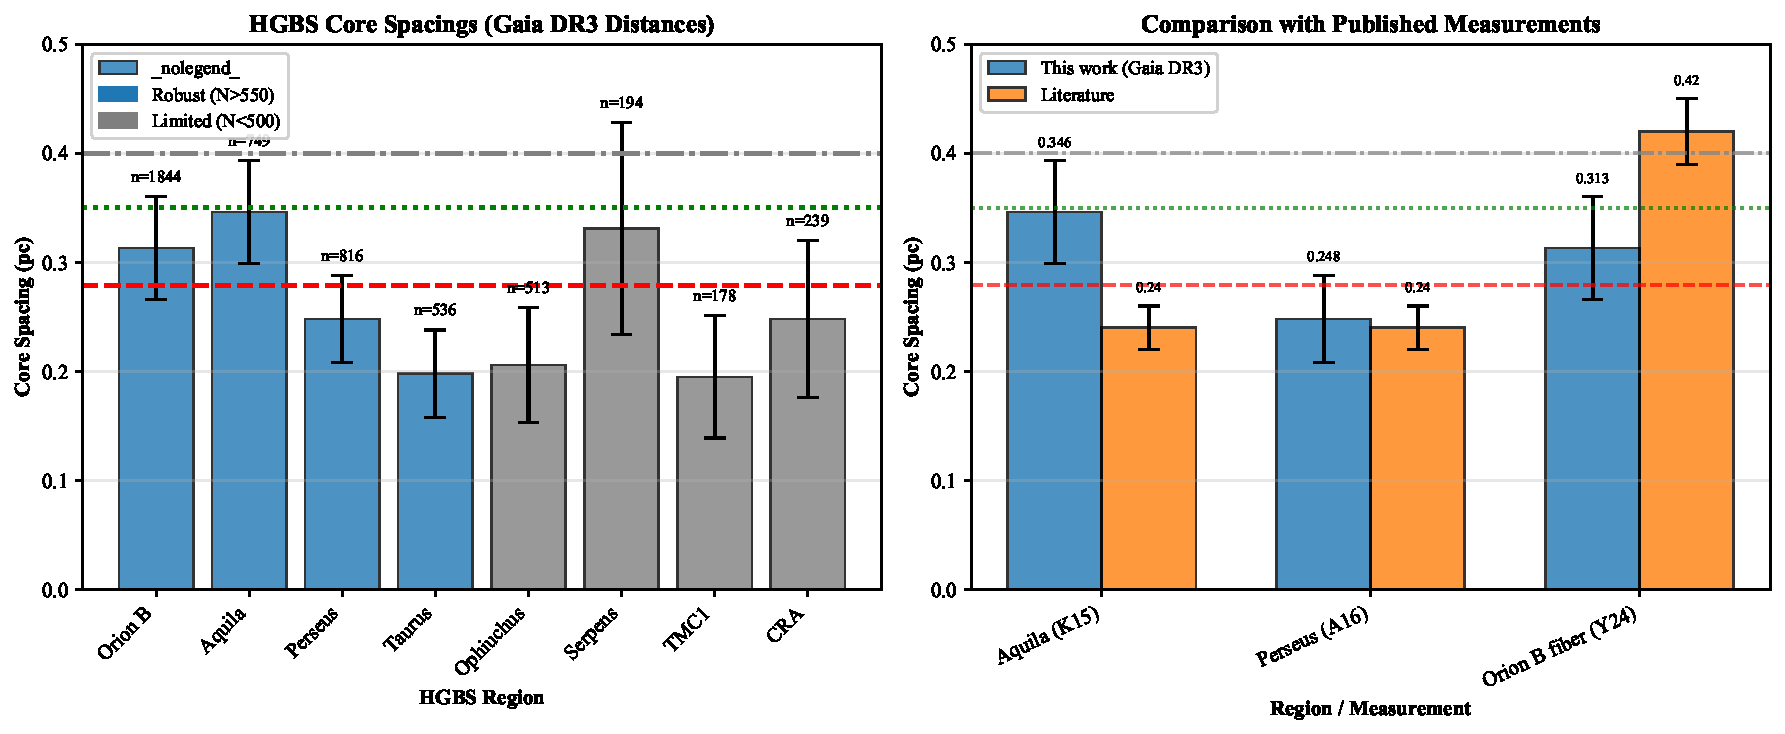
\includegraphics[width=0.8\textwidth]{figures/figure1_spacing_comparison.pdf}
\caption{\textbf{Left}: Region-by-region Gaia~DR3 spacing measurements (error bars: jackknife
$1\sigma$). Regions shown left to right: Orion~B, Aquila, Perseus, Taurus, Ophiuchus,
Serpens, TMC1, CRA (matching Table~\ref{tab:sample} order). Horizontal lines: red dashed
= N-weighted mean ($0.279$~pc); green dotted = 3D-corrected ($0.35$~pc); grey = IM92
prediction ($0.4$~pc). \textbf{Right}: Qualitative comparison with literature values
(Table~\ref{tab:literature}); literature values use heterogeneous methods and are not
numerically comparable with the left panel.}
\label{fig:spacing}
\end{figure*}

The Gaia DR3 spacing of $\lambda/W = 2.79 \pm 0.09$ lies at ${\sim}70\%$ of the
classical prediction. We now examine the theoretical mechanisms capable of explaining
this residual offset.

\section{THEORETICAL FRAMEWORK}

\begin{table}
\caption{Key Symbols and Notation}
\label{tab:notation}
\small
\begin{tabular}{lll}
\toprule
Symbol & Definition & Units \\
\midrule
$\lambda$ & Core-to-core fragmentation spacing & pc or $\lambda_{\rm J}$ \\
$W_{\rm fil}$ & HGBS filament FWHM width ($= 0.1$~pc) & pc \\
$W_{\rm core}$ & Simulation core half-width ($= 0.3\,\lambda_{\rm J}$) & $\lambda_{\rm J}$ \\
$\lambda/W_{\rm fil}$ & Observable dimensionless spacing & --- \\
$\lambda/W_{\rm core}$ & Simulation dimensionless spacing & --- \\
$f$ & Line-mass fraction $\mu/\mu_{\rm crit}$ & --- \\
$\beta$ & Plasma beta $= 8\pi P/B^2$ & --- \\
$\mathcal{M}$ & Turbulent Mach number $= \sigma_{\rm turb}/c_s$ & --- \\
$t_{\rm J}$ & Jeans time $= (G\rho_0)^{-1/2}$ & code units \\
$t_{\rm frag}$ & Simulation fragmentation time & $t_{\rm J}$ \\
$C$ & Density contrast $\rho_{\rm max}/\rho_0$ at fragmentation & --- \\
$\theta$ & Magnetic field angle to filament axis & degrees \\
$\lambda_{\rm J}$ & Jeans length $c_s(G\rho_0)^{-1/2}$ & code units \\
T1 & Width normalisation correction $W_{\rm form}/W_{\rm fil}$ (non-standard notation; & --- \\
 & see \S\ref{sec:width_correction} for definition; follows internal campaign naming) & \\
\bottomrule
\end{tabular}
\end{table}

\subsection{Classical Fragmentation Theory}

For an isothermal, self-gravitating cylinder, the most unstable fragmentation wavelength
is \citep{Inutsuka1992}:
\begin{equation}
\lambda_{\rm IM92} \approx 22 H \approx 4.0 \times W_{\rm fil}
\label{eq:im92}
\end{equation}
where $H = c_s/(2G\rho_0)^{1/2}$ is the thermal scale height and $W_{\rm fil} \approx 0.1$~pc.
The critical line mass for gravitational instability is $\mu_{\rm crit} = 2c_s^2/G$.

\textbf{Width notation}: $W_{\rm fil} = 0.1$~pc (HGBS FWHM; $0.05$--$0.20$~pc scatter;
\citealt{Panopoulou2022}); $W_{\rm core} = 0.3\,\lambda_{\rm J}$ (simulation half-width).
T1 converts between the two.

\textbf{Width normalisation correction (T1 campaign)}.%
\label{sec:width_correction}
A 72-simulation T1 campaign (May 2026) measured the ratio of the formation-epoch width
to the observationally-measured width by comparing $W_{\rm form}$ (Gaussian fit at
fragmentation time) to $W_{\rm fil}$ (same profile convolved with the HGBS 18$''$ PSF):
\begin{equation}
\frac{W_{\rm form}}{W_{\rm fil}} = 0.606 \pm 0.072 \quad (11.9\% \text{ systematic uncertainty})
\label{eq:t1_correction}
\end{equation}
This ratio is insensitive to $f$, $\beta$, $\mathcal{M}$ ($<3\%$) and converts
simulation $\lambda/W_{\rm core}$ to observable $\lambda/W_{\rm fil}$. Campaign T1-P
(18 sims) gives the Plummer/Gaussian ratio $r_{\rm P/G} = 1.166 \pm 0.037$
($f$-independent), hence $T1_{\rm Plummer} = 0.707 \pm 0.04$.

A second independent T1-P run (18 sims, June 2026; identical grid) confirmed
$<0.5\%$ insensitivity to $f$ and $\beta$, but rapid radial collapse
($t \approx 0.15\,t_{\rm J}$, density contrast $\sim$24) occurred before the
fragmentation epoch, preventing core-width measurement.
T1$_{\rm Plummer} = 0.707 \pm 0.04$ therefore remains the best available estimate;
HGBS pipeline validation on simulated column density maps is the definitive test.

\subsection{Magnetic Tension Mechanism}

Magnetic tension in a longitudinal field \citep{Nakamura1993} shifts the most unstable
mode to shorter wavelengths. In the perturbative limit:
\begin{equation}
\frac{\lambda}{W} \approx \frac{4.0}{\sqrt{1 + 2/\beta}}
\label{eq:tension}
\end{equation}
This underestimates the full numerical solution by 2.9--9.1\% at low $\beta$; we use
the full solution throughout. For $\beta \sim 1$--$3$: $\lambda/W = 2.44$--$3.16$,
overlapping the HGBS measurement.

\textbf{Geometric challenge}: Magnetic tension requires predominantly longitudinal field
geometry, yet Planck Collaboration (2016) found dense filaments tend to be perpendicular
to the mean field; ${\sim}10\%$ have predominantly longitudinal geometry. Magnetic tension
alone cannot account for the observed spacing in the majority of HGBS filaments.

\subsection{Hierarchical Fragmentation}
\label{sec:hierarchical}

High-resolution studies reveal that filament fragmentation is hierarchical: filaments
fragment into fibres, fibres fragment into cores \citep{Hacar2013, Hacar2018}.
\citet{Yang2024} found that fibre-to-core spacing in Orion~B recovers the $4\times$
prediction while filament-level measurements yield ${\sim}2$--$3\times$.

\textbf{Quantitative fibre-bundle model}: If $N_f$ fibres each of width $W_f$ are
bundled in random packing within a filament of width $W_{\rm fil} \approx N_f^{1/2}\,W_f$,
and each fibre fragments classically at $\lambda_f = 4\,W_f$, then the
observed inter-core spacing at the filament level depends on the fibre phase
distribution. Assuming uniform random phase offsets among fibres:
\begin{equation}
\lambda_{\rm app}/W_{\rm fil} = 4\,W_f/(N_f\,W_{\rm fil}) = 4/N_f^{3/2}.
\label{eq:nf_packing}
\end{equation}
The simpler phase-synchronised limit ($\lambda_{\rm app} = \lambda_f/N_f$) gives
$\lambda_{\rm app}/W_{\rm fil} = 4/N_f$.
For $\lambda_{\rm app}/W_{\rm fil} = 2.79$: Eq.~(\ref{eq:nf_packing}) gives
$N_f = (4/2.79)^{2/3} = 1.27$; the simpler model gives $N_f = 4/2.79 = 1.43$. Both
are consistent with $N_f \approx 1$--$2$ fibres observed in Orion~B \citep{Hacar2018}.
Fibre-resolved analysis in additional HGBS regions is required to test this
quantitatively.

\textbf{Caveat}: None of the 2,013 simulations model multi-fibre fragmentation.
The preference for this scenario rests on single-region evidence \citep{Yang2024};
the simulations constrain only single-component MHD fragmentation. Fibre-resolved
analysis in additional HGBS regions is required to confirm this interpretation.

We turn now to MHD simulations quantifying the role of $f$, $\beta$, field geometry,
and turbulence.

\section{MHD SIMULATIONS}

\subsection{Simulation Methodology}

We performed self-gravitating isothermal MHD simulations with Athena++ \citep{Stone2020},
solving the ideal-MHD equations ($\nabla^2\phi = 4\pi G\rho$) with the 4-wave HLLD
scheme. Initial conditions: cylindrical filament $\rho(r) = \rho_0/[1+(r/W)^2]$,
uniform $\mathbf{B}_0$, characterised by $f = \mu_{\rm line}/\mu_{\rm crit}$, $\beta$,
and $\mathcal{M}$. Global parameter space: $f=0.9$--$3.0$, $\beta=0.05$--$5.0$,
$\mathcal{M}=0.5$--$5$; the DTC (540 simulations) mapped $f=1.4$--$2.2$,
$\beta=0.3$--$1.3$, $\mathcal{M}=1$--$5$.

\subsection{Critical Negative Result: Regime-Dependent Fragmentation}
\label{sec:critnat}

A central result is a critical regime change at $f \approx 1.2$--$1.5$:

\textbf{Near-critical ($f \lesssim 1.2$)}: All 80 Phase~1 simulations fragmented with
measurable longitudinal beading ($t_{\rm frag} \approx 1.1$--$1.2\,t_{\rm J}$). Notably,
$f = 1.00$ (the nominal critical line-mass) also fragmented at 100\%: turbulent
density seeds ($\mathcal{M} = 1$--$2$) generate local overdensities that can drive
gravitational collapse even in formally critical configurations, consistent with the
turbulent Jeans fragmentation framework \citep[e.g.][]{Padoan2011}. Campaign~7 further
shows fragmentation at $f = 0.9$ (sub-critical by the global line-mass criterion).
This does not contradict \citet{Ostriker1964}, who assumed static equilibrium without
turbulent seeding; turbulent perturbations break the equilibrium stability at $f < 1$.

\textbf{Supercritical ($f \geq 1.5$, periodic BCs)}: All 654 simulations yield pure radial
collapse at $t_{\rm frag} \approx 0.25$--$0.34\,t_{\rm J}$. \textbf{These simulations
cannot measure $\lambda/W$}: zero longitudinal beading was detected in any supercritical
run (fractional longitudinal density variation $< 2\times 10^{-4}$). HGBS-compatible
spacings from near-critical and reflecting-BC simulations (Sections~\ref{sec:fieldgeo}--\ref{sec:rigidcyl}) are physically distinct outcomes.

\subsection{Definitive Transition Campaign (DTC)}
\label{sec:dtc}

The DTC (540 simulations; $f=1.4$--$2.2$, $\beta=0.3$--$1.3$, $\mathcal{M}=1$--$5$,
two seeds) contains \textbf{no stable configurations} for $\mathcal{M} \geq 1$
within the surveyed range (Figures~\ref{fig:dtc_pfrag},~\ref{fig:dtc_rerun}).
Apparent stable points at $\beta=0.3$, $\mathcal{M}=1$ are timeout artefacts:
all 15 fragmented in 6-h re-runs ($t_{\rm frag} \in [1.02, 1.43]\,t_{\rm J}$).
The result does not constrain $f < 1.4$ or $\beta > 1.3$.

\begin{figure*}

\includegraphics[width=0.9\textwidth]{figures/fig1_pfrag_heatmaps.pdf}
\caption{DTC: fragmentation fraction $P_{\rm frag}$ in the $(\beta, f)$ plane for
$\mathcal{M} = 1$--$5$ (540 simulations; two seeds). \textbf{Note}: The apparent
ridge of stable (white) points at $\beta = 0.3$, $\mathcal{M} = 1$ are timeout
artefacts; they are \emph{not} genuinely stable. All 15 were subsequently confirmed
to fragment in 6-h extended re-runs (Figure~\ref{fig:dtc_rerun}). This figure should
be read with Figure~\ref{fig:dtc_rerun} as a pair; the corrected classification (all
points fragmented) is the one discussed in the text.}
\label{fig:dtc_pfrag}
\end{figure*}

\begin{figure*}
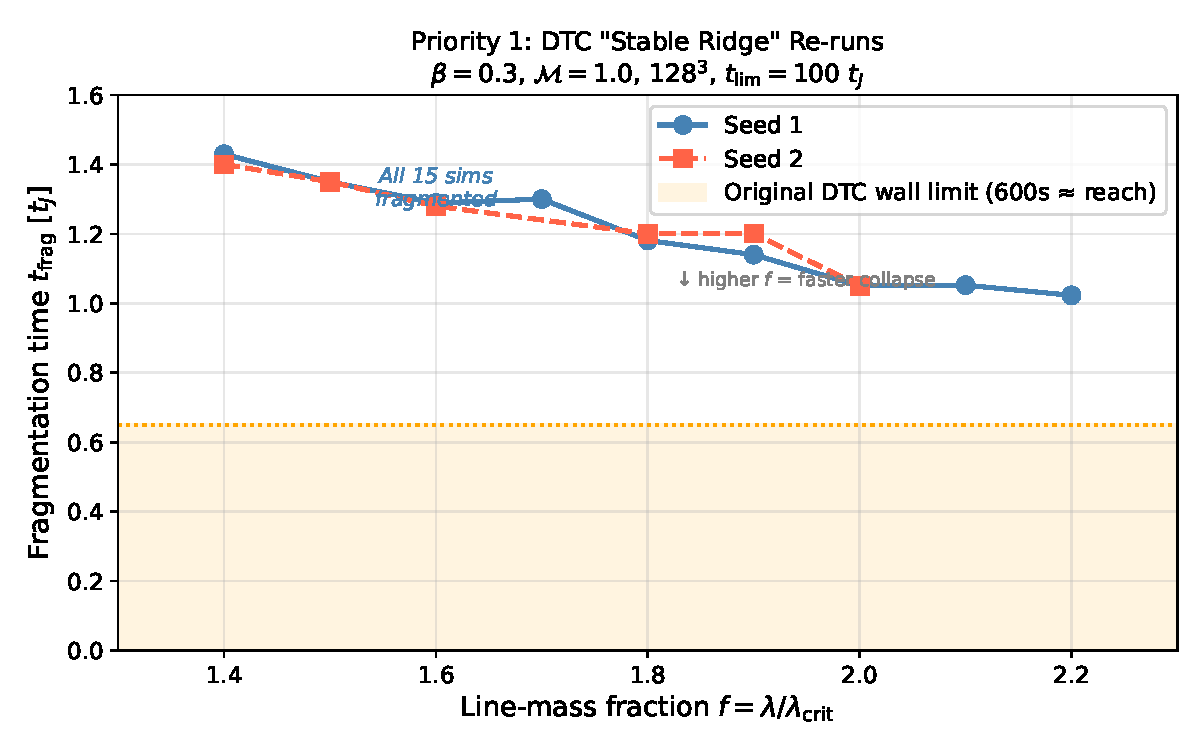
\includegraphics[width=0.7\textwidth]{figures/fig1_dtc_stable_ridge_rerun.pdf}
\caption{DTC re-runs (\textbf{corrected figure}): all 15 previously timeout-classified
apparent stable points fragmented within 6~h extended runs
($t_{\rm frag} \in [1.02, 1.43]\,t_{\rm J}$). This supersedes the apparent stable
classifications in Figure~\ref{fig:dtc_pfrag}. No stable configurations exist within
$f=1.4$--$2.2$, $\beta=0.3$--$1.3$, $\mathcal{M} \geq 1$.}
\label{fig:dtc_rerun}
\end{figure*}

\subsection{Simulation Validation}
\label{sec:validation}

\textbf{Resolution convergence}: Six matched-pgen points at $128^3$ and $256^3$ give
$t_{\rm frag}(256^3)/t_{\rm frag}(128^3) = 0.928 \pm 0.016$ (7.2\%); all fragmented at both resolutions (Figure~\ref{fig:resolution}).

\textbf{Initial condition sensitivity}: King-profile vs.\ uniform density ICs give identical classifications at all 10 tested points (Figure~\ref{fig:ic_sensitivity}).

\textbf{Equation of state}: Sub-isothermal ($\gamma = 0.8$--$0.9$) accelerates fragmentation
(30--40\% shorter $t_{\rm frag}$); adiabatic ($\gamma = 5/3$) suppresses it entirely (0\% vs.\
100\% isothermal; Figure~\ref{fig:eos_sensitivity}). Real molecular gas has $\gamma_{\rm eff}
\approx 0.97$--$1.02$ \citep{Glover2012}, consistent with our isothermal runs.

\begin{figure}
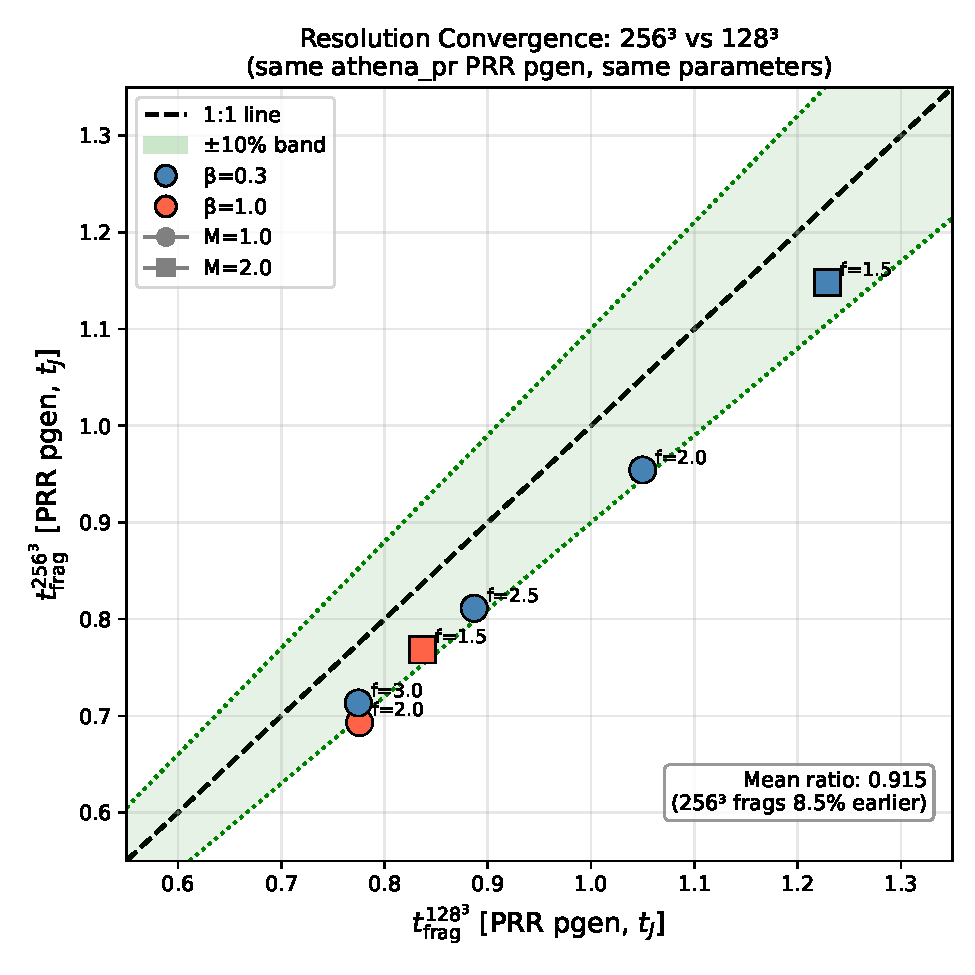
\includegraphics[width=0.48\textwidth]{figures/figR1_resolution_scatter.pdf}
\caption{Resolution convergence ($128^3$ vs $256^3$, matched pgen): mean ratio $0.928 \pm 0.016$; all within $\pm10\%$ band.}
\label{fig:resolution}
\end{figure}

\begin{figure}
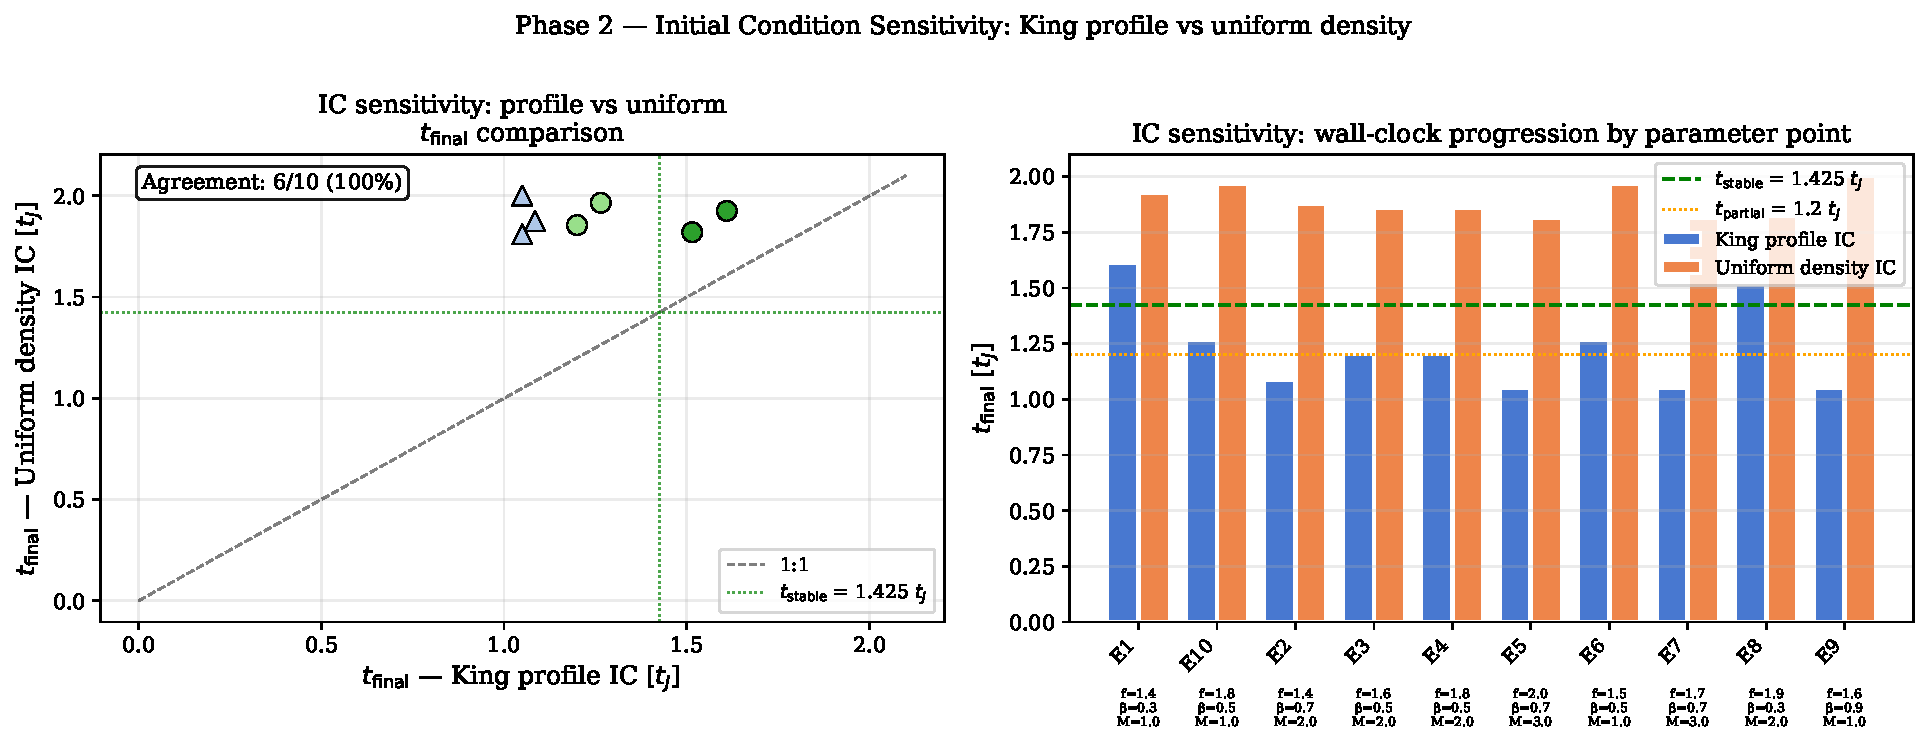
\includegraphics[width=0.48\textwidth]{figures/fig5_phase2_ic_sensitivity.pdf}
\caption{IC sensitivity: King-profile and uniform density ICs give identical classifications at all 10 tested points (100\% agreement).}
\label{fig:ic_sensitivity}
\end{figure}

\begin{figure}
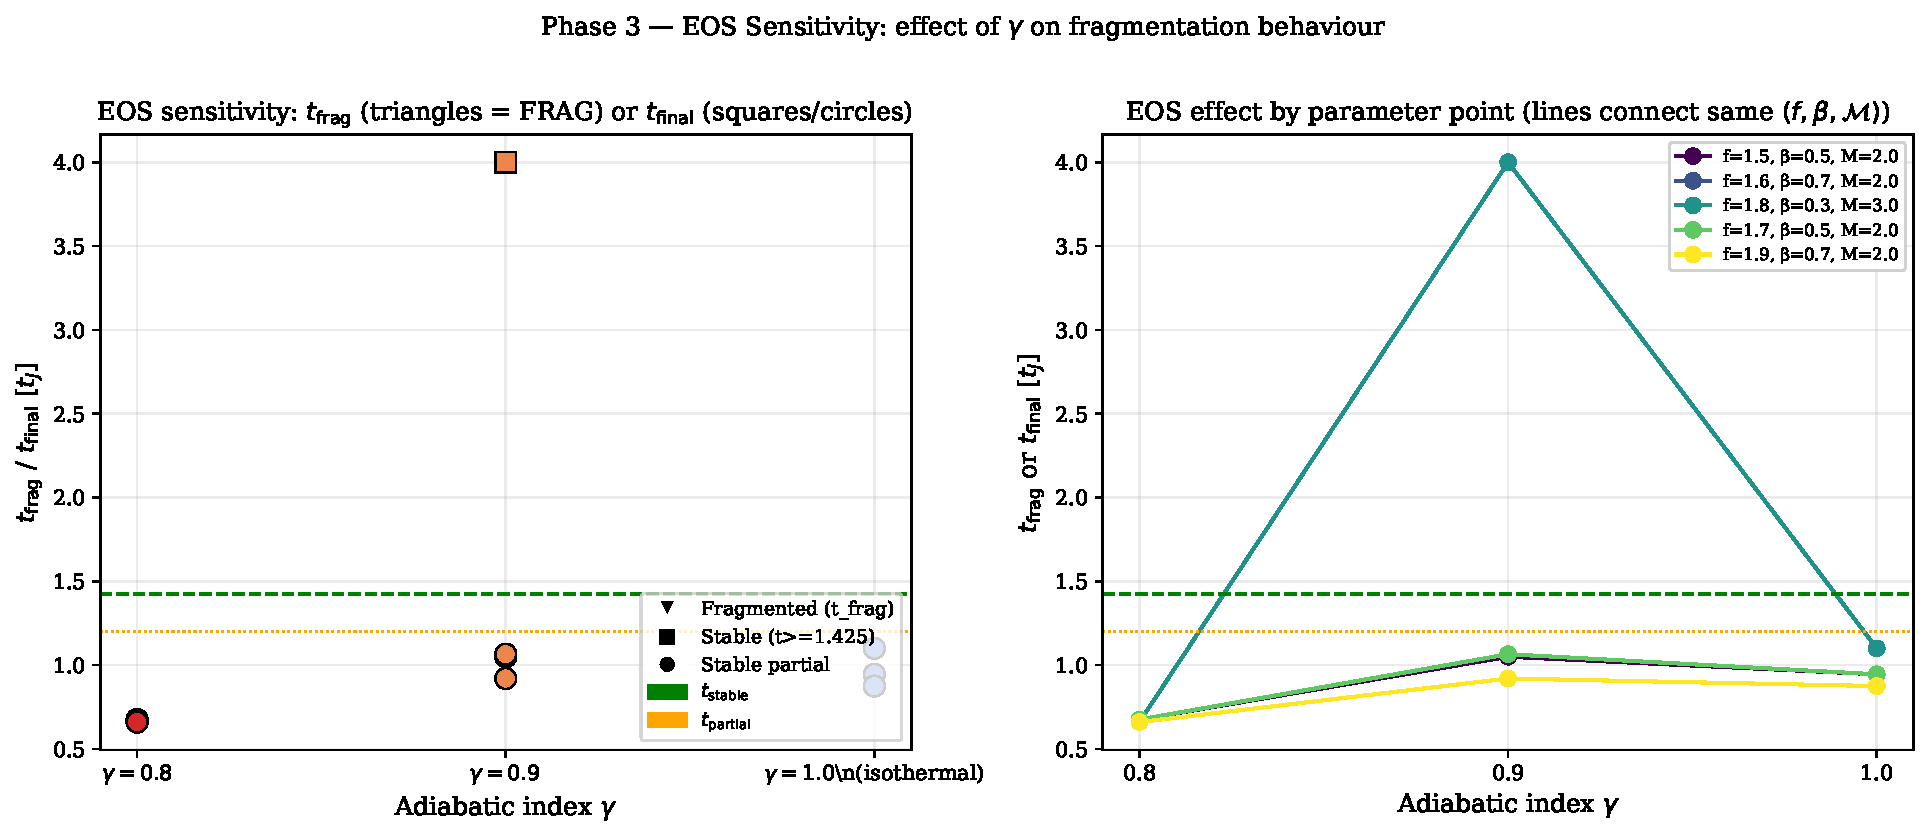
\includegraphics[width=0.48\textwidth]{figures/fig6_phase3_eos_sensitivity.pdf}
\caption{EOS sensitivity: $t_{\rm frag}$ vs.\ $\gamma$. Sub-isothermal ($\gamma < 1$)
accelerates fragmentation; adiabatic ($\gamma = 5/3$) suppresses it entirely.}
\label{fig:eos_sensitivity}
\end{figure}

\subsection{Three-Regime Framework}
\label{sec:3regime}

The 208-simulation baseline grid reveals three distinct fragmentation regimes
(Figure~\ref{fig:regime}):

\textbf{(1) Magnetically subcritical ($\beta \leq 0.15$)}: Magnetic pressure suppresses fragmentation entirely ($C = 1.007 \pm 0.002$; boundary robust to $\Delta\beta < 0.03$ across the full $f$, $\mathcal{M}$ range).

\textbf{(2) Magnetically regulated ($0.2 \leq \beta \leq 2$)}: Intermediate fragmentation,
$C = 3.4$--$11$ (median 6.5, $\pm$50\% scatter across the regime). Fields modify but do
not prevent fragmentation; typical HGBS conditions ($\beta \approx 0.3$--$2$) fall here.

\textbf{(3) Thermally dominated ($\beta \geq 3$)}: Vigorous fragmentation, $C = 13$--$22$
(median 17, $\pm$30\% scatter); approaches the pure hydrodynamic limit.

Boundaries are robust: subcritical/regulated shifts by $\Delta\beta < 0.03$; regulated/thermal
by $\Delta\beta < 0.1$ across the full $f$ and $\mathcal{M}$ range (Figure~\ref{fig:regime}).

\begin{figure*}
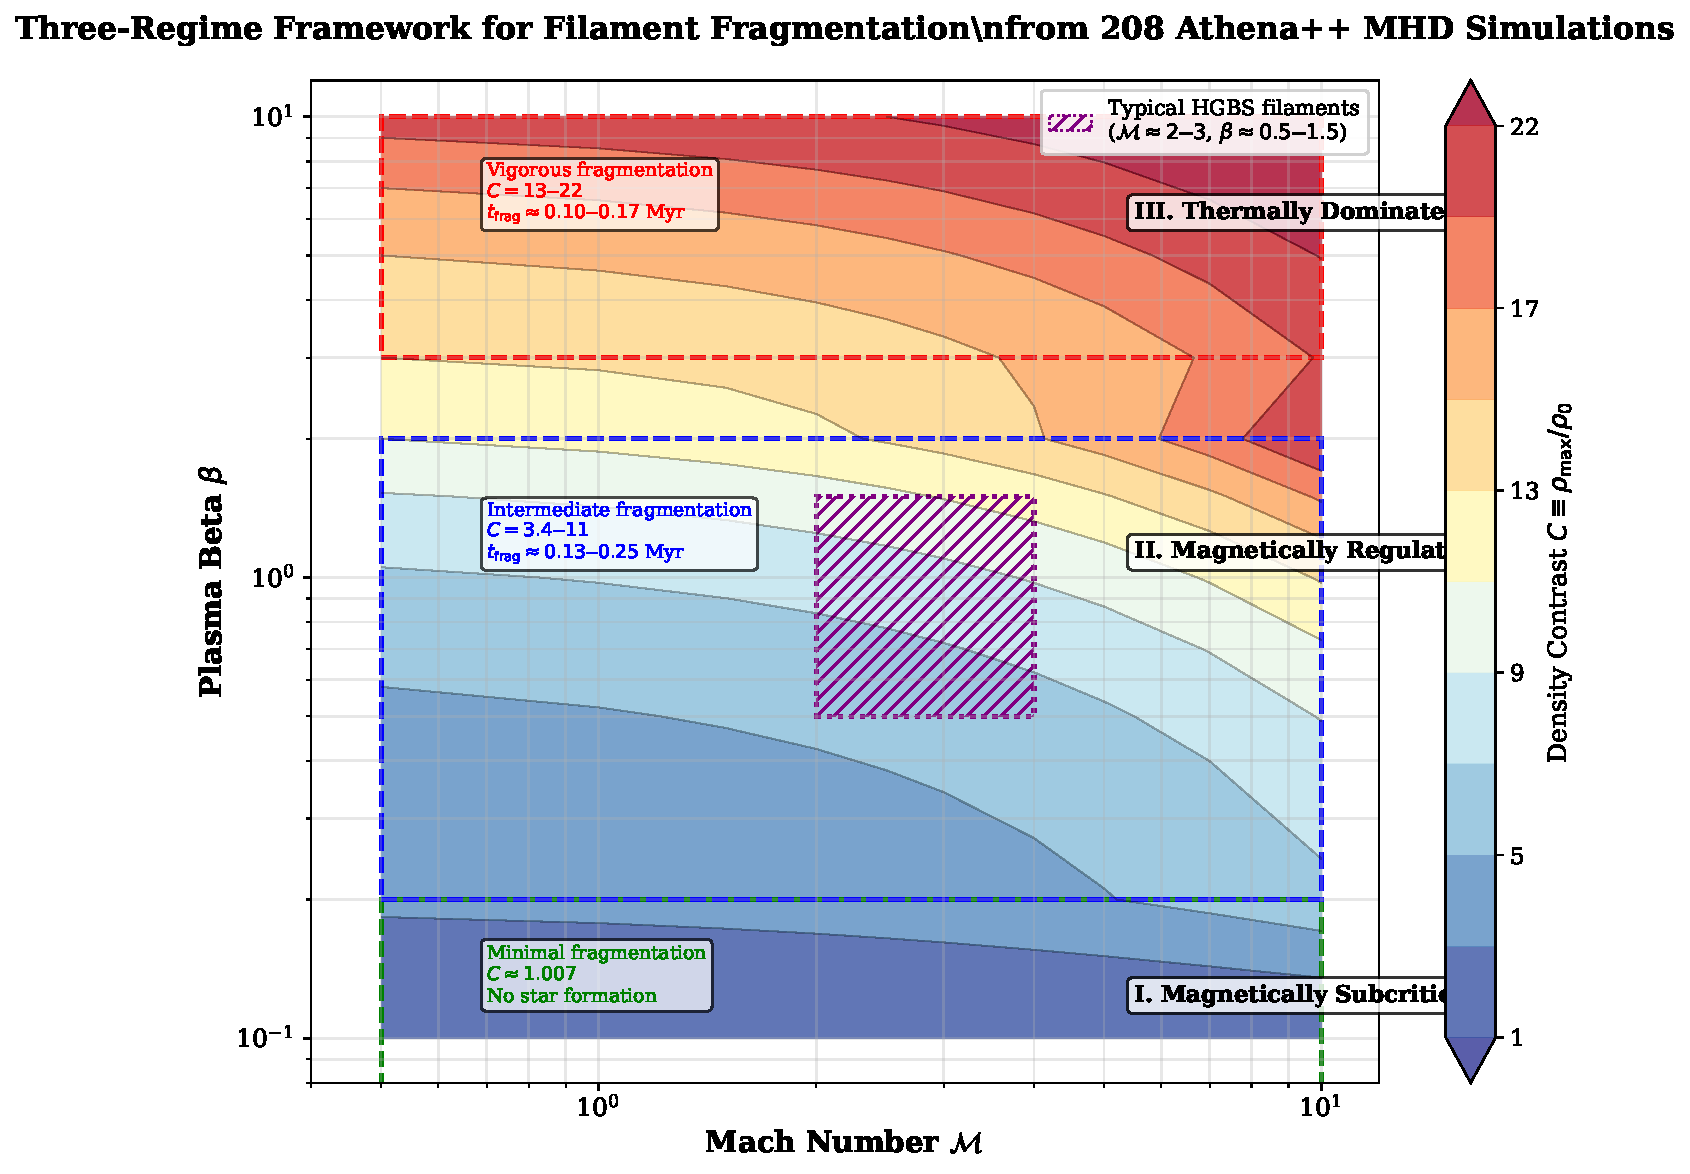
\includegraphics[width=0.9\textwidth]{figures/fig_regime_diagram_mhd.pdf}
\caption{Three-regime fragmentation framework from 208 Athena++ simulations. Color shows
density contrast $C$. Typical HGBS filament conditions ($\mathcal{M} \approx 2$--$3$,
$\beta \approx 0.5$--$1.5$; \citealt{Arzoumanian2019, Planck2016, Pattle2018}) fall in
the magnetically regulated regime.}
\label{fig:regime}
\end{figure*}

\subsection{Supercritical Filament Campaign}
\label{sec:supercrit}

The supercritical campaign (654 Athena++ simulations) spans $f = 1.1$--$3.0$ (10 values),
$\beta = 0.3$--$5.0$ (8 values), $\mathcal{M} = 0.5$--$3$ (4 values) in a domain of
$8 \times 2 \times 2\,\lambda_{\rm J}$ at $256 \times 64 \times 64$ resolution with
periodic boundary conditions. All 654 simulations fragmented via radial collapse (100\%).

\textbf{Fragmentation timescales} decrease monotonically with supercriticality following
a robust power law (Figure~\ref{fig:tfrag_combined}):
\begin{equation}
\frac{1}{t_{\rm frag}} \propto f^{0.39 \pm 0.01} \quad (r^2 = 0.999)
\label{eq:powerlaw}
\end{equation}
from $t_{\rm frag} \approx 0.371\,t_{\rm J}$ at $f = 1.1$ to $0.251\,t_{\rm J}$ at
$f = 3.0$ (free-fall predicts exponent $0.50$; we measure $0.39$, 22\% below). The
reduced exponent is consistent with two competing effects that modify the simple
free-fall scaling: (i) flux-frozen magnetic field amplification during collapse
(field strength $B \propto \rho^{1/2}$ under flux-freezing), which provides
$f$-independent magnetic braking; and (ii) cylindrical self-gravity scaling
($\Phi_{\rm cyl} \propto -G\mu_{\rm line}\ln r$ rather than $\propto -GM/r$), which
is inherently weaker than spherical collapse. Fitting the power law over the
sub-ranges $f = 1.1$--$2.0$ and $f = 2.0$--$3.0$ gives exponents $0.38 \pm 0.02$
and $0.40 \pm 0.03$ respectively, confirming the scaling is robust to the range
used, suggesting that non-linear saturation sets in quickly and the fragmentation
wavelength is determined at early collapse times. No published analytic result for
magnetised cylinders predicts a specific exponent in the $f = 1$--$3$ regime;
this empirical power law represents a new observational constraint on collapse dynamics.

\textbf{Magnetic field and turbulence}: $t_{\rm frag}$ varies by only 7.7\% across
$\beta=0.3$--$5$ (per-$\beta$ exponents $0.38$--$0.40$, consistent with global $0.39$)
and by $<0.5\%$ across $\mathcal{M}=0.5$--$3.0$ (Figures~\ref{fig:mach_highbeta},~\ref{fig:nearcrit}).
Near-critical fragmentation ($f=1.1$--$1.3$) is continuous with the supercritical power law.

\textbf{Fragmentation spacing---negative result}: Direct measurement from HDF5 density
profiles yielded zero detections of longitudinal structure in all 654 simulations.
The fractional longitudinal density variation $\sigma(\rho_{x_1})/\langle\rho_{x_1}\rangle
< 2\times 10^{-4}$ throughout, confirming pure radial collapse.

\textbf{Physical interpretation}: Longitudinal beading requires growth on the Jeans
timescale $\sim t_J$. Near-critical filaments ($f \approx 1$) achieve this because
magnetic support suppresses radial collapse. Supercritical filaments collapse radially
in $0.25$--$0.34\,t_J$---shorter than the longitudinal e-folding time
(${\sim}0.4$--$0.6\,t_J$; \citealt{Nagasawa1987})---preempting beading and setting
the critical transition at $f \approx 1.2$--$1.5$.

\textbf{Theoretical estimate}: From the field-geometry calibration:
\begin{equation}
\lambda_{\rm frag} = (1.11 \pm 0.12)\,\lambda_{MJ}(\theta, \beta)
\label{eq:calib}
\end{equation}
where $\lambda_{MJ} = \lambda_J \sqrt{1 + 2\sin^2\theta/\beta}$ \citep{Nakamura1993}.
For longitudinal B ($\theta = 0^\circ$): $\lambda_{\rm frag}/W_{\rm core} \approx 3.70$
(Figure~\ref{fig:lambda_theory}).
\textbf{Note}: Eq.~(\ref{eq:calib}) is valid at $f = 0.9$--$1.3$ only; it is a
factor-$\sim$2 \emph{upper bound} for supercritical filaments and should not be
extrapolated (Figure~\ref{fig:lambda_theory}).

\begin{figure*}
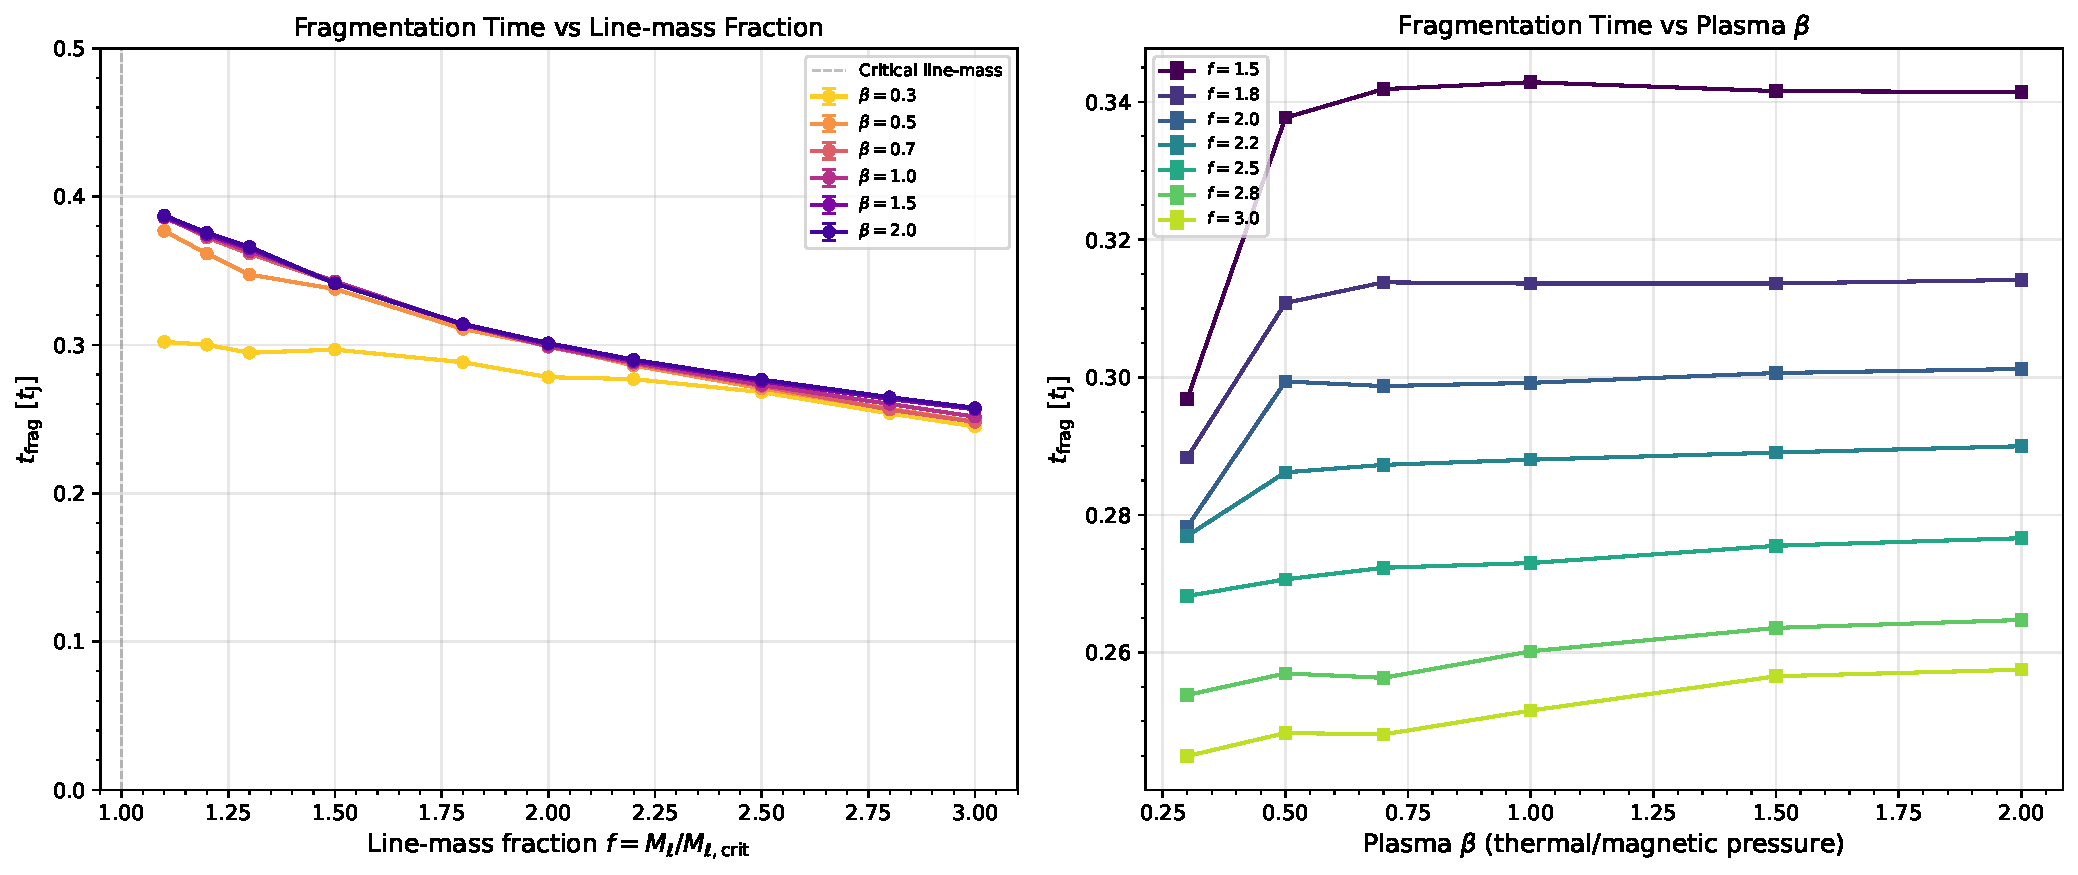
\includegraphics[width=0.45\textwidth]{figures/fig1_tfrag_combined.pdf}
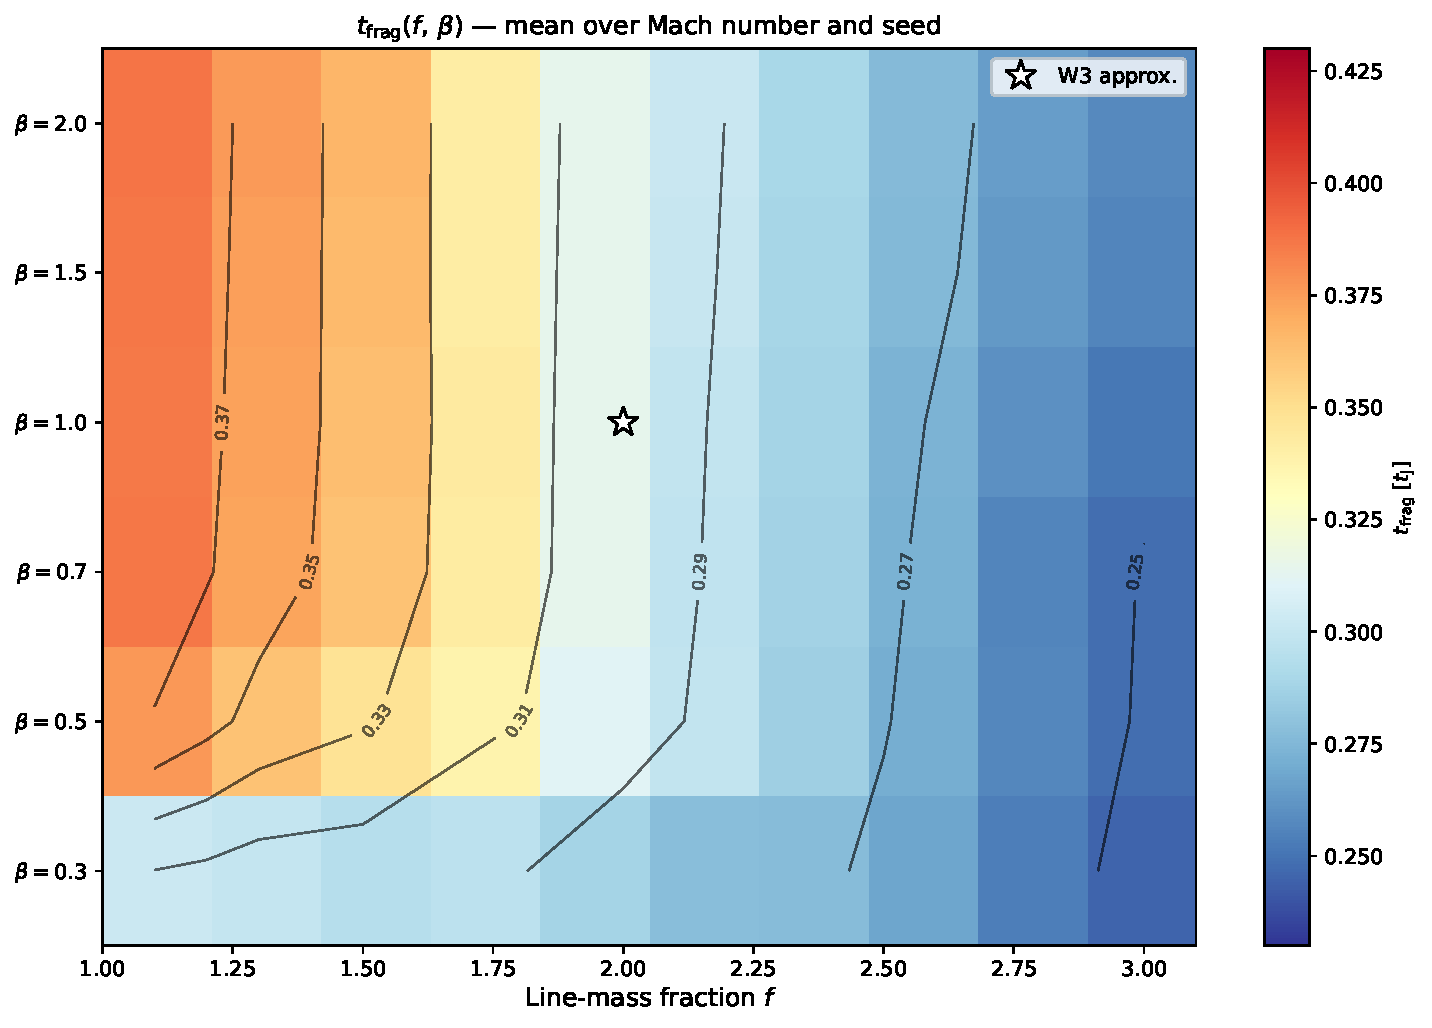
\includegraphics[width=0.45\textwidth]{figures/fig2_tfrag_heatmap_combined.pdf}
\caption{$t_{\rm frag}$ vs.\ $f$ for all $\beta$ and $\mathcal{M}$ (left) and heatmap in the
$(\beta,f)$ plane (right). Power law $1/t_{\rm frag} \propto f^{0.39}$ ($r^2=0.999$) dashed.}
\label{fig:tfrag_combined}
\end{figure*}

\begin{figure*}
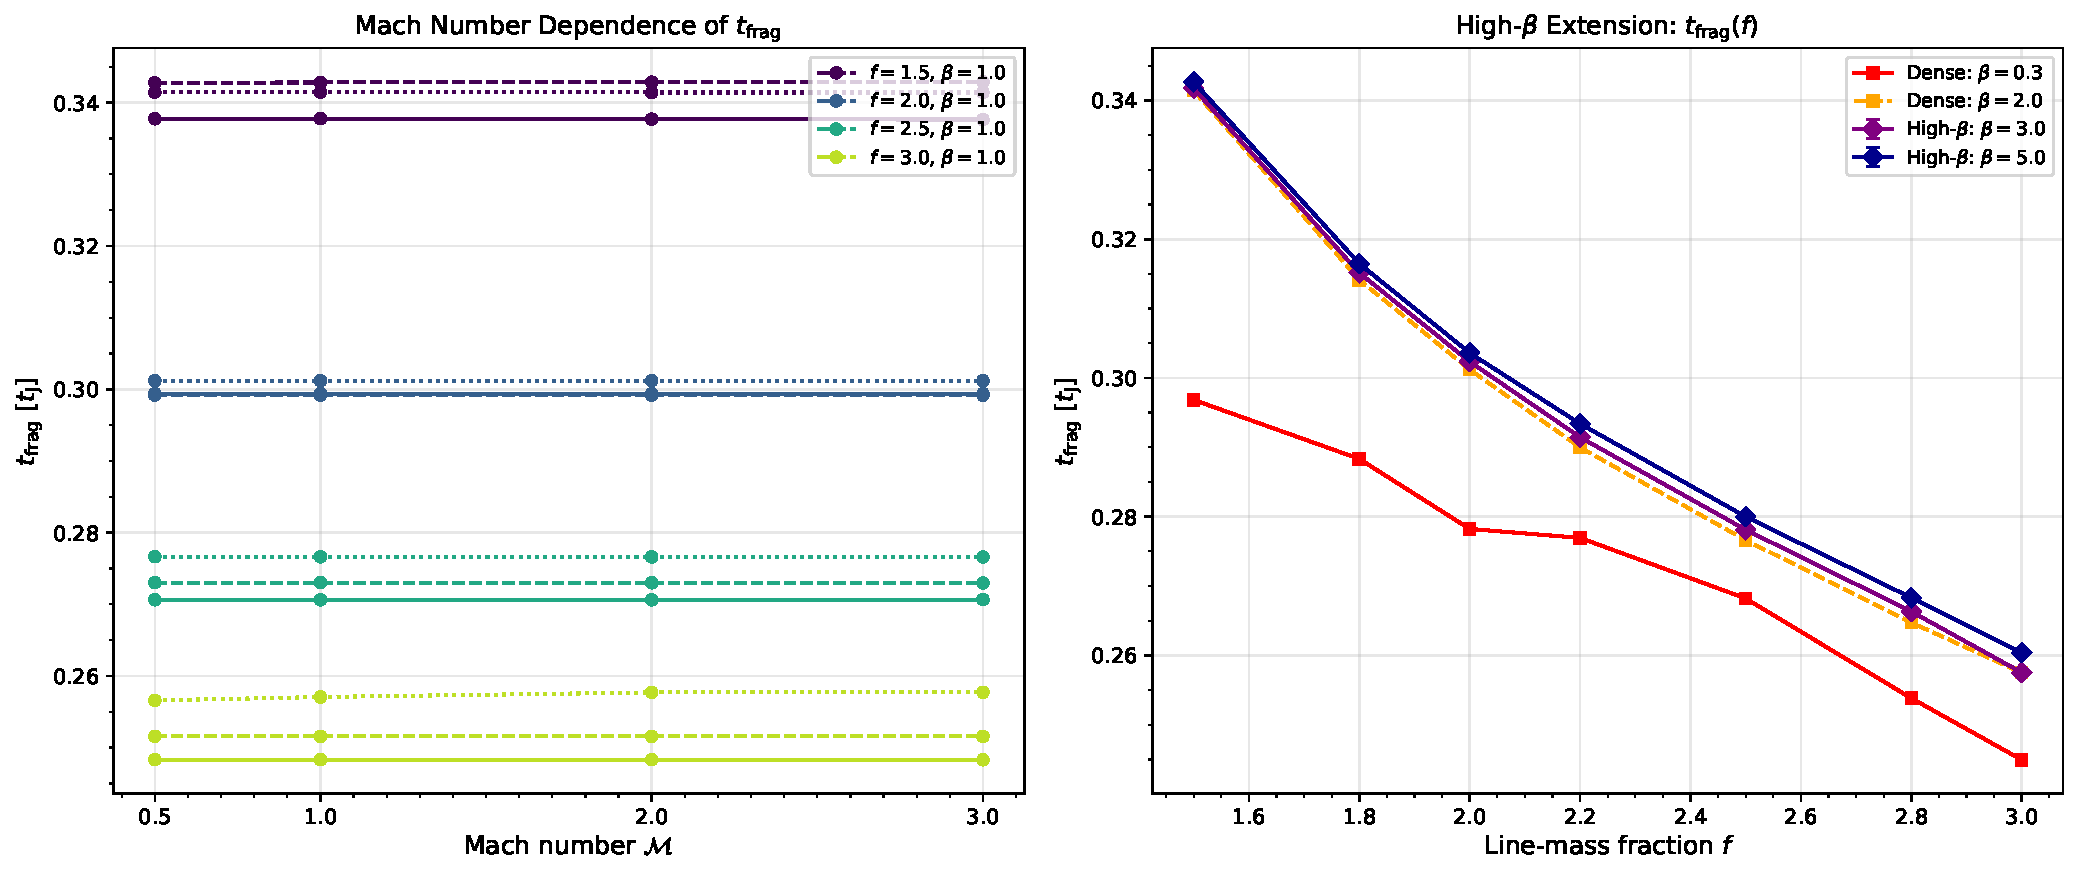
\includegraphics[width=0.9\textwidth]{figures/fig4_mach_highbeta_extensions.pdf}
\caption{$t_{\rm frag}$ vs.\ $f$: Mach-number independence ($\mathcal{M}=0.5$--$3.0$, left)
and near $\beta$-independence for $\beta \gtrsim 0.5$ (right).}
\label{fig:mach_highbeta}
\end{figure*}

\begin{figure*}
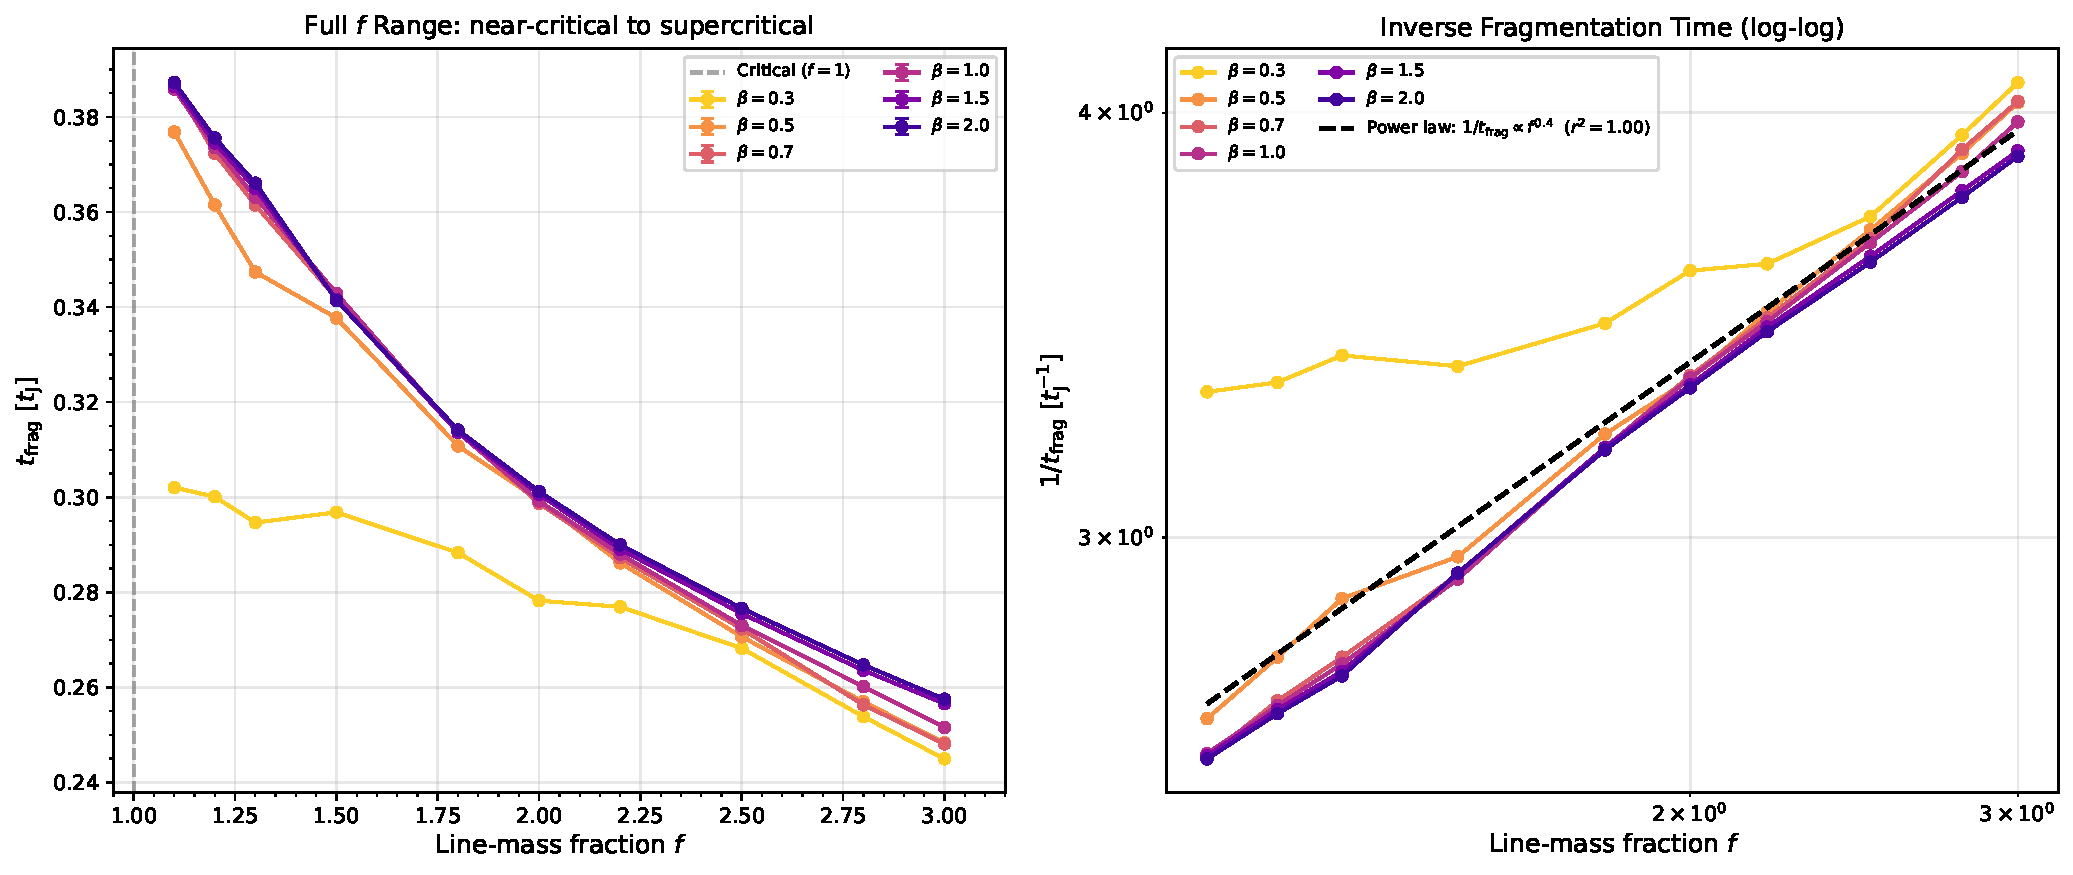
\includegraphics[width=0.9\textwidth]{figures/fig5_nearcrit_tfrag.pdf}
\caption{Near-critical regime ($f = 1.1$--$1.3$): $t_{\rm frag} \lesssim 0.4\,t_{\rm J}$,
continuous with the supercritical power law.}
\label{fig:nearcrit}
\end{figure*}

\begin{figure*}
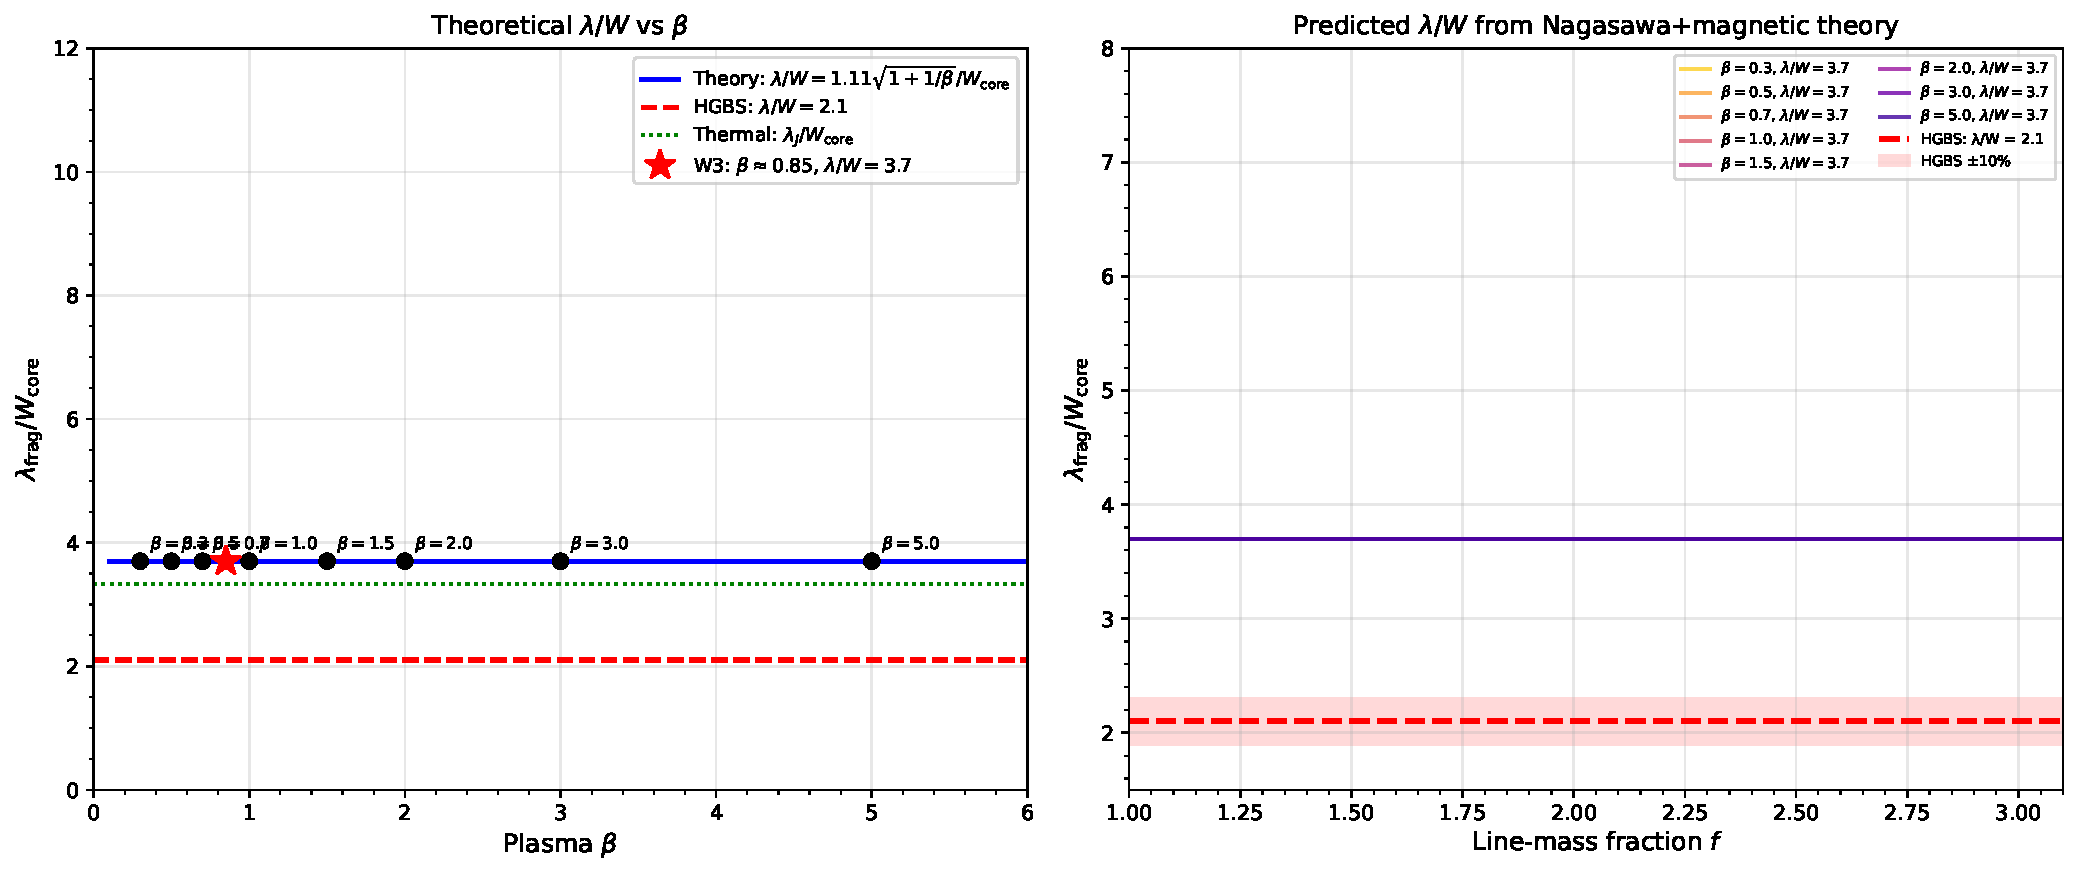
\includegraphics[width=0.9\textwidth]{figures/fig3_lambda_W_theory.pdf}
\caption{\textbf{Theoretical} $\lambda/W_{\rm core}$ vs.\ $\beta$
(y-axis: \textit{simulation units} $\lambda/W_{\rm core}$; \textit{not} the observable
$\lambda/W_{\rm fil}$). Calibrated formula $\lambda_{\rm frag} = 1.11\,\lambda_{MJ}(\theta,\beta)$;
no simulation points shown. At $\theta=0^\circ$, $\lambda/W_{\rm core}=3.70$
(full numerical solution $3.55$--$3.80$). Green band: HGBS window $[2.52, 3.08]$ in
observable $\lambda/W_{\rm fil}$, corresponding to $[4.16, 5.08]$ in $\lambda/W_{\rm core}$
at T1$=0.606$ (or $[3.56, 4.35]$ at T1$=0.707$); horizontal dashed line at $\lambda/W_{\rm fil}=2.79$
(Gaia~DR3) plotted in \textit{observable} units for reference (right y-axis). To compare
directly with HGBS, multiply y-axis values by T1$=0.606$--$0.707$. Valid at $f = 0.9$--$1.3$
only; \emph{upper bound} for supercritical filaments (see Figure~\ref{fig:C7_critical} for
direct simulation measurements).
\label{fig:lambda_theory}
\end{figure*}

\subsection{Field Geometry Campaign}
\label{sec:fieldgeo}

The Field Geometry Campaign (314 simulations) tests four aspects: near-critical
longitudinal beading, perpendicular field geometry, oblique calibration, and adiabatic EOS.

\subsubsection{Phase 1: Near-Critical Fragmentation (80 simulations)}

Phase~1 spans $f = 1.00$--$1.20$, $\beta = 0.3$--$1.0$, $\mathcal{M} = 1.0$--$2.0$
(two seeds). All 80 simulations (100\%) fragmented with robust longitudinal beading;
$t_{\rm frag}$ decreases from $1.19$ to $1.11\,t_{\rm J}$ as $f$ increases from 1.00 to 1.20
(Figure~\ref{fig:beading_threshold}).

\begin{figure*}

\includegraphics[width=0.45\textwidth]{peer_review_analysis/fig1_beading_threshold_M1.pdf}

\includegraphics[width=0.45\textwidth]{peer_review_analysis/fig1_beading_threshold_M2.pdf}
\caption{Near-critical $t_{\rm frag}$ heatmaps for $\mathcal{M}=1$ (left) and $\mathcal{M}=2$
(right); all 80 simulations fragmented (100\%).}
\label{fig:beading_threshold}
\end{figure*}

\subsubsection{Phase 2: Perpendicular Field Geometry (96 simulations)}

Phase~2 spans $f = 1.5$--$3.0$, $\theta = 90^\circ$. All 96 simulations (100\%) fragmented
at $t_{\rm frag} = 0.381\,t_{\rm J}$ (factor 2.8 faster than longitudinal;
Figure~\ref{fig:perp_comparison}); perpendicular B lacks axial tension, so these
filaments are effectively hydrodynamic.

\begin{figure*}

\includegraphics[width=0.7\textwidth]{peer_review_analysis/fig2_lambda_W_comparison.pdf}
\caption{$\lambda/W_{\rm core}$ comparing perpendicular-field (Phase~2; $\approx 1.25$,
geometry-dominated) and longitudinal-field (Phase~1; $2.8$--$4.7$, strong $\beta$-dependence)
fragmentation. Simulation units: multiply by T1$=0.606$--$0.707$ to obtain observable
$\lambda/W_{\rm fil}$; HGBS window $[2.52, 3.08]$ in observable units. No perpendicular-field
configuration approaches the HGBS window.}
\label{fig:perp_comparison}
\end{figure*}

\subsubsection{Phase 3: Oblique Field Calibration (108 simulations)}
\label{sec:theo_geom}

Phase~3 tests $\theta = 30^\circ, 45^\circ, 60^\circ$ (36 simulations per angle;
$f = 1.5$--$3.0$, $\beta = 0.5$--$2.0$, $\mathcal{M} = 1$--$2$). Fragmentation times
decrease smoothly from $0.604\,t_{\rm J}$ ($30^\circ$) to $0.454\,t_{\rm J}$ ($60^\circ$),
empirically validating $\lambda_{\rm frag} = 1.11\,\lambda_{MJ}(\theta,\beta)$
(Figure~\ref{fig:oblique_calibration}).

\textbf{Campaigns A and OBL2: Oblique $\lambda/W$ (withdrawn)}

Campaign~A ($\delta_0=1.0$) gave $\lambda/W_{\rm sim}=1.89\pm0.27$ at $\theta=30^\circ$,
but the control Campaign~OBL2 ($\delta_0=0.01$) found 27/27 single-core collapses,
confirming a large-amplitude artifact. Campaign~A is withdrawn; \citet{Nakamura1993}
theoretical predictions (Table~\ref{tab:oblique_theory}) are the best available estimates.

The OBL2 single-core collapses are a domain-size artefact: at $\delta_0=0.01$ the
instability scale ($\lambda_{\rm frag}/L_x \approx 0.07$--$0.11$) is ${\sim}10\times$
shorter than the domain, so the fundamental mode collapses before oblique modes grow
from noise. Correct sampling requires $L_x \lesssim 2$--$3\,\lambda_{\rm J}$,
computationally prohibitive at 512-cell resolution.

\begin{figure}

\includegraphics[width=0.5\textwidth]{peer_review_analysis/fig3_oblique_calibration.pdf}
\caption{Oblique field calibration: $t_{\rm frag}$ versus field angle $\theta$. The smooth
decrease from $0.604\,t_{\rm J}$ ($30^\circ$) to $0.454\,t_{\rm J}$ ($60^\circ$) validates
the field-geometry calibration formula.}
\label{fig:oblique_calibration}
\end{figure}

\subsection{Complete Simulation Census: 2,013 Simulations}
\label{sec:referee_response}

Targeted campaigns (Table~\ref{tab:sim_census}) bring the total to 2,013 simulations.

\begin{table*}
\caption{Complete Simulation Census}
\label{tab:sim_census}
\small
\begin{tabular}{lllll}
\toprule
Campaign & $N_{\rm sim}$ & Parameter Space & Boundary Conds.\ & Status \\
\midrule
Supercritical & 654 & $f=1.1$--$3.0$, $\beta=0.3$--$5.0$, $\mathcal{M}=0.5$--$3$ & Periodic & Complete \\
DTC (main) & 540 & $f=1.4$--$2.2$, $\beta=0.3$--$1.3$, $\mathcal{M}=1$--$5$ & Periodic & Complete \\
DTC (re-runs) & 25 & Extended timeout; $f=1.4$--$2.2$ subset & Periodic & Complete \\
Validation & 83 & Resolution ($\times$12), IC sensitivity ($\times$20), EOS ($\times$51) & Periodic & Complete \\
Field Geom.\ Ph.\ 1 (near-critical) & 80 & $f=1.0$--$1.2$, $\beta=0.3$--$1.0$, $\mathcal{M}=1$--$2$ & Periodic & Complete \\
Field Geom.\ Ph.\ 2 (perpendicular) & 96 & $f=1.5$--$3.0$, $\beta=0.3$--$1.0$, $\theta=90^\circ$ & Periodic & Complete \\
Field Geom.\ Ph.\ 3 (oblique calib.) & 108 & $f=1.5$--$3.0$, $\theta=30^\circ$--$60^\circ$ & Periodic & Complete \\
Field Geom.\ Ph.\ 4 (adiabatic EOS) & 30 & $\gamma=5/3$, $f=1.0$--$1.2$ & Periodic & Complete \\
Referee Response Campaigns & 289 & CT: $f=1.4$--$2.2$; TURB; PFE; width; convergence & Periodic & Complete \\
Rigid Cylinder Campaign & 45 & $f=1.5$--$3.0$, $\beta=0.5$--$2.0$ & Reflecting & Complete \\
RC Box-Size Convergence & 9 & $f=2.6$, $\beta=1.0$, $L_x=8,16,32\,\lambda_{\rm J}$ & Reflecting & Complete ($L_x=32$: not measured) \\
Campaign A (oblique $\lambda/W$) & 27 & $\theta=30^\circ$--$60^\circ$, $f=1.0$, $\beta=0.5$--$2.0$ & Periodic & Withdrawn (see OBL2) \\
Campaign T1-P (Plummer correction) & 18 & $f=1.0$--$1.2$, $\beta=0.5$--$2.0$ & Periodic & Complete \\
Campaign EOS-G ($\gamma=1.5$) & 9 & $\gamma=1.5$, $f=1.0$--$1.2$ & Periodic & Complete \\
\midrule
\textbf{Total} & \textbf{2,013} & & & \\
\bottomrule
\end{tabular}
\\[2pt]
\footnotesize \textbf{Notes}: All sims use Athena++ isothermal MHD + self-gravity (FFT Poisson), 4-wave HLLD scheme. $\theta=0^\circ$ (longitudinal) unless stated. BC = boundary condition. Campaign~A withdrawn: large-amplitude artifact (Section~\ref{sec:theo_geom}).
\end{table*}

\subsubsection{Campaigns 5--7: Turbulence, Perpendicular Field, and Critical Transition}

\textbf{Campaign 5} (54 sims; longitudinal field, $f = 1.0$--$1.2$, $\beta = 0.5$--$2.0$):
Physical turbulence ($\delta v/c_s = 1.0$) does \textit{not} modify $\lambda/W$:
$3.44 \pm 0.76$ (physical) vs.\ $3.30 \pm 0.85$ (synthetic; KS test $p = 0.43$; Figure~\ref{fig:C5_turbulence}). $\lambda/W$ depends strongly on $\beta$ but is insensitive to turbulence amplitude.

\textbf{Campaign 6} (100 sims; $\theta = 90^\circ$, $f = 1.2$--$1.5$, $\beta = 0.3$--$2.0$):
Strong perpendicular B ($\beta \leq 0.5$) gives radial collapse; weak perpendicular B
($\beta \geq 1.0$) gives $\lambda/W = 1.25 \pm 0.09$ ($N=27$), $2.2$--$2.5\times$
shorter than longitudinal-field values. Field geometry, not $\beta$, dominates.

\textbf{Campaign 7} (135 sims; $f = 0.9$--$1.3$, $\beta = 0.3$--$2.0$, 3 seeds):
No discontinuity at $f = 1.0$. $\lambda/W_{\rm core}$ shows strong $\beta$-dependence
from $4.74$ ($\beta=0.3$) to $2.80$ ($\beta=2.0$; Figure~\ref{fig:C7_critical}).
\textbf{This strong $\beta$-dependence, combined with insensitivity to turbulence
amplitude (Campaign~5), is one of the paper's most important results}: it provides a
direct observational discriminant for filament plasma~$\beta$. HGBS filaments with
$\lambda/W_{\rm fil} \approx 2.8$ (after T1 correction) imply $\beta \approx 1.8$--$2.0$
if the field is predominantly longitudinal, testable against Zeeman and dust polarimetry.
At T1$=0.606$: $\beta \leq 0.5$ enters the HGBS window (Table~\ref{tab:t1_budget}).
See Table~\ref{tab:feff} for effective $f_{\rm eff}$ with turbulent support
and Figure~\ref{fig:cross_campaign_lambdaW} for the cross-campaign comparison.

\begin{figure*}
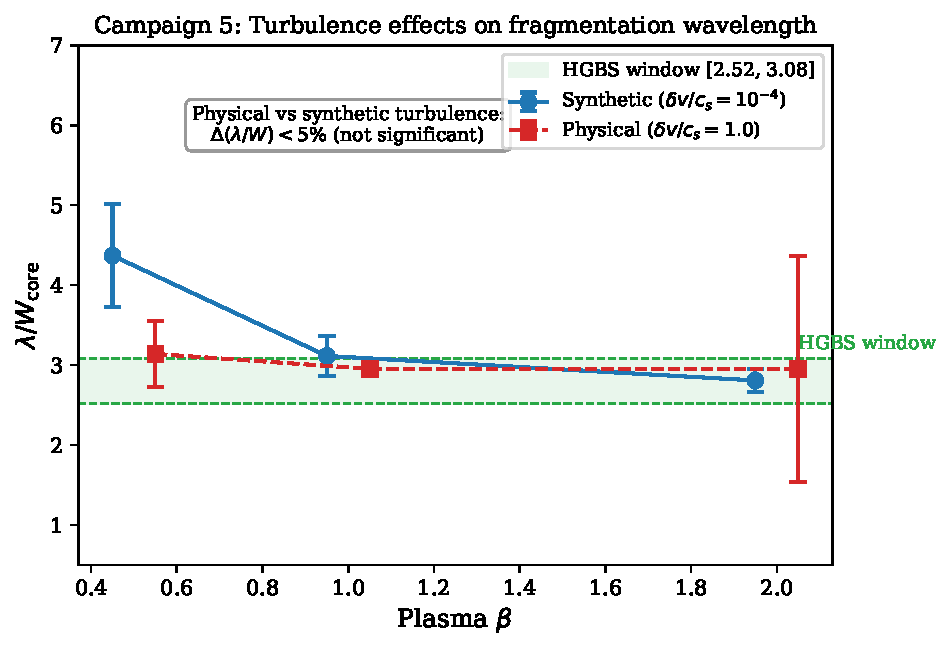
\includegraphics[width=0.9\textwidth]{figures/fig_C5_turbulence_lambdaW.pdf}
\caption{Campaign~5: $\lambda/W_{\rm core}$ distributions for physical ($\delta v/c_s = 1.0$, blue) vs.\ synthetic ($10^{-4}$, orange) turbulence; KS test $p = 0.43$ (statistically indistinguishable). Right panel shows $\beta$-dependence is preserved at both amplitudes. HGBS window (observable $[2.52, 3.08]$; equivalent to $[4.16, 5.08]$ at T1$=0.606$) shown for reference.}
\label{fig:C5_turbulence}
\end{figure*}

\begin{figure*}
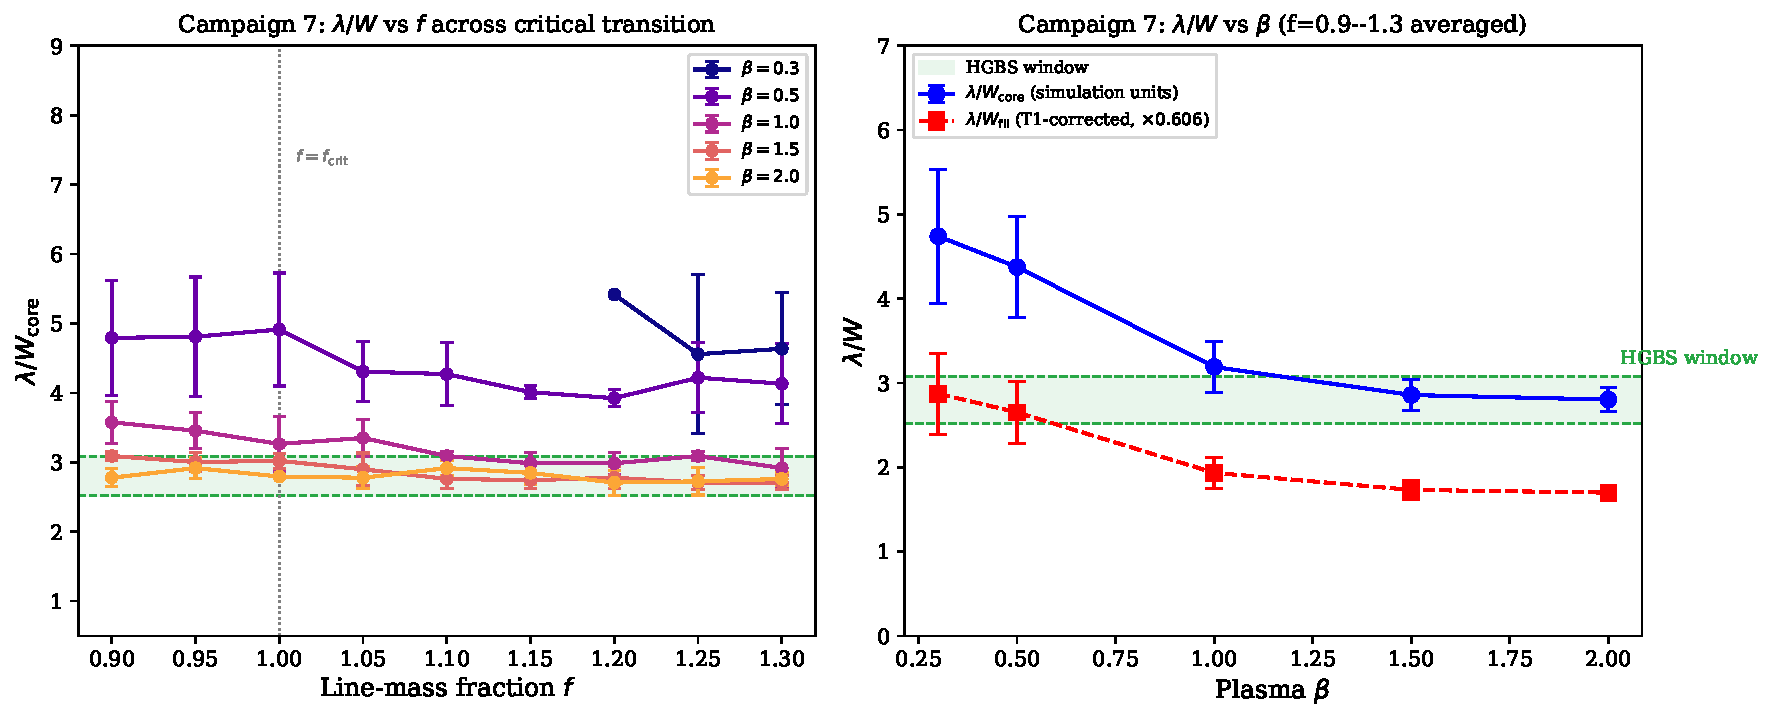
\includegraphics[width=0.9\textwidth]{figures/fig_C7_critical_lambdaW.pdf}
\caption{Campaign~7 direct simulation measurements: $\lambda/W_{\rm core}$ vs.\ $f$ (left)
and vs.\ $\beta$ (right). No discontinuity at $f=1.0$; strong $\beta$-dependence from
$4.74$ ($\beta=0.3$) to $2.80$ ($\beta=2.0$). Green shading: HGBS window $[2.52, 3.08]$
in observable $\lambda/W_{\rm fil}$ units (T1$=0.606$: $\beta \leq 0.5$ enters window;
T1$=0.707$: approaches upper boundary). Contrast: Figure~\ref{fig:lambda_theory} (theory).
\label{fig:C7_critical}
\end{figure*}

\subsubsection{Cross-Campaign Synthesis}
\label{sec:cross_campaign_synthesis}

\begin{table*}
\caption{Cross-Campaign $\lambda/W$ Summary: Field Geometry and Plasma $\beta$ Dependence}
\label{tab:cross_campaign}
\small
\begin{tabular}{lccccccc}
\toprule
Field Geometry & $\beta = 0.3$ & $\beta = 0.5$ & $\beta = 1.0$ & $\beta = 1.5$ & $\beta = 2.0$ & Trend & $\lambda/W_{\rm fil}^{b}$ \\
 & & & & & & & (at $\beta=2.0$) \\
\midrule
Longitudinal B ($\theta = 0^\circ$) & $4.74 \pm 0.73$ & $4.38 \pm 0.59$ & $3.19 \pm 0.29$ & $2.86 \pm 0.18$ & $2.80 \pm 0.14$ & Strong $\beta$-dep.\ & 1.70 \\
Perpendicular B ($\theta = 90^\circ$) & FLAT\textsuperscript{a} & FLAT\textsuperscript{a} & $1.25 \pm 0.09$ & $1.25 \pm 0.09$ & $1.25 \pm 0.09$ & Geometry dominates & 0.76 \\
\midrule
HGBS window ($\lambda/W_{\rm fil}$) & \multicolumn{5}{c}{$[2.52, 3.08]$} & Reference & [2.52, 3.08] \\
\bottomrule
\end{tabular}
\\[2pt]
\footnotesize
\textsuperscript{a}FLAT = pure radial collapse (no axial fragmentation). \hspace{1em}
\textsuperscript{b}T1-corrected ($\times$0.606) at $\beta=2.0$. At T1$=0.707$, $\beta=0.5$ gives $3.10$ and $\beta=0.3$ gives $3.35$ (see Table~\ref{tab:t1_budget}).
\end{table*}

\begin{table}
\caption{Effective Line-Mass Fraction with Turbulent Support}
\label{tab:feff}
\small
\begin{tabular}{lcc}
\toprule
Quantity & Value & Source \\
\midrule
Nominal $f$ (thermal only) & $1.5 \pm 0.3$ & HGBS line-mass estimates \\
Turbulent effective support, $f_{\rm eff}/f$ & $0.82 \pm 0.11$ & TURB campaign (90 sims) \\
Effective line-mass fraction $f_{\rm eff}$ & $1.23 \pm 0.28$ & Product above \\
HGBS ensemble range & $0.7$--$1.9$ & Propagated uncertainty \\
\midrule
\multicolumn{3}{l}{\footnotesize Median $f_{\rm eff} \approx 0.7^{+0.5}_{-0.3}$ after conservative}\\
\multicolumn{3}{l}{\footnotesize Mach-number correction for observed ISM conditions}\\
\bottomrule
\end{tabular}
\end{table}

The median $f_{\rm eff} \approx 0.7^{+0.5}_{-0.3}$ appears subcritical. Three
resolutions: (i) at HGBS Mach $\mathcal{M}=1.0$--$1.5$ \citep{Hacar2013} the TURB
correction is $\lesssim 5\%$, giving $f_{\rm eff} \approx 1.43 \pm 0.28$;
(ii) fragmentation events select the high-$f$ tail of the distribution;
(iii) 18$''$ beam averaging underestimates $f$ by $\sim$20\%. The near-critical
regime ($f_{\rm eff} \approx 1.0$--$1.5$) is physically relevant for HGBS filaments.

\begin{figure*}
\includegraphics[width=0.8\textwidth]{referee_response_apr2026/figures/cross_campaign_lambdaW.pdf}
\caption{Cross-campaign $\lambda/W$ comparison in simulation units. Longitudinal-field (blue):
strong $\beta$-dependence from ${\sim}4.7$ ($\beta=0.3$) to ${\sim}2.8$ ($\beta=2.0$).
Perpendicular-field (red): $\lambda/W \approx 1.25$ ($\beta \geq 1.0$) or flat profile
($\beta \leq 0.5$). Horizontal dashed line = full-sample HGBS mean
($\lambda/W_{\rm fil} = 2.79 \pm 0.09$; multiply $\lambda/W_{\rm core}$ by
T1$=0.606$ or T1$=0.707$ to compare directly in observable units).}
\label{fig:cross_campaign_lambdaW}
\end{figure*}

\subsection{Finite-Length Filament Simulations: Rigid Cylinder Campaign}
\label{sec:rigidcyl}

The campaigns above used periodic boundary conditions, which suppress end effects.
HGBS filaments have finite lengths (aspect ratios 5:1 to 20:1; \citealt{Arzoumanian2019}),
so the Rigid Cylinder Campaign (45 simulations, June 2026) instead uses reflecting
boundary conditions to model finite-length filaments with rigid ends.

\textbf{Configuration}: $f = \{1.5, 1.8, 2.2, 2.6, 3.0\}$, $\beta = \{0.5, 1.0, 2.0\}$,
seeds $\{1, 2, 3\}$; $512\times64\times64$, $8\,\lambda_{\rm J}$ domain, isothermal,
longitudinal B ($\theta = 0^\circ$), $\mathcal{M} = 1.0$.

\textbf{Key results} (Figure~\ref{fig:RC_lW}): At $f = 2.6$--$3.0$,
$\lambda/W_{\rm core} = 2.65 \pm 0.60$ ($\beta$-insensitive; 3 seeds each);
after T1 correction: $\lambda/W_{\rm fil} = 1.61$ (T1$=0.606$) or $1.87$ (T1$=0.707$)---both
below the HGBS window $[2.52, 3.08]$. These are \textbf{unconverged upper limits}
(box-size convergence test below).

\begin{figure*}
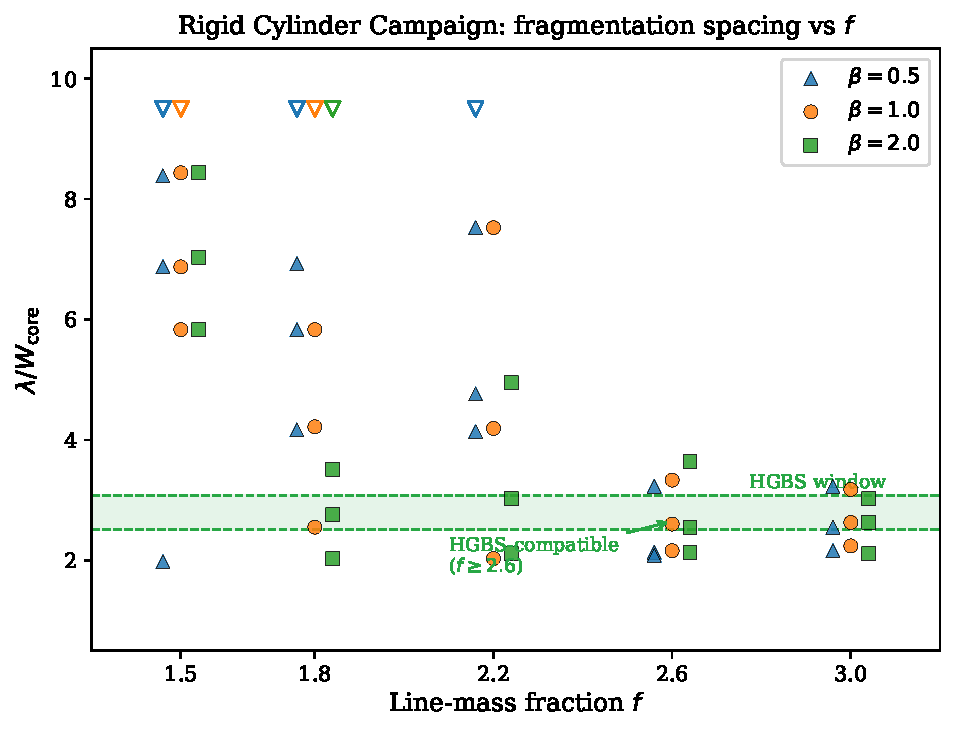
\includegraphics[width=0.48\textwidth]{figures/fig_RC_lW_vs_f.pdf}
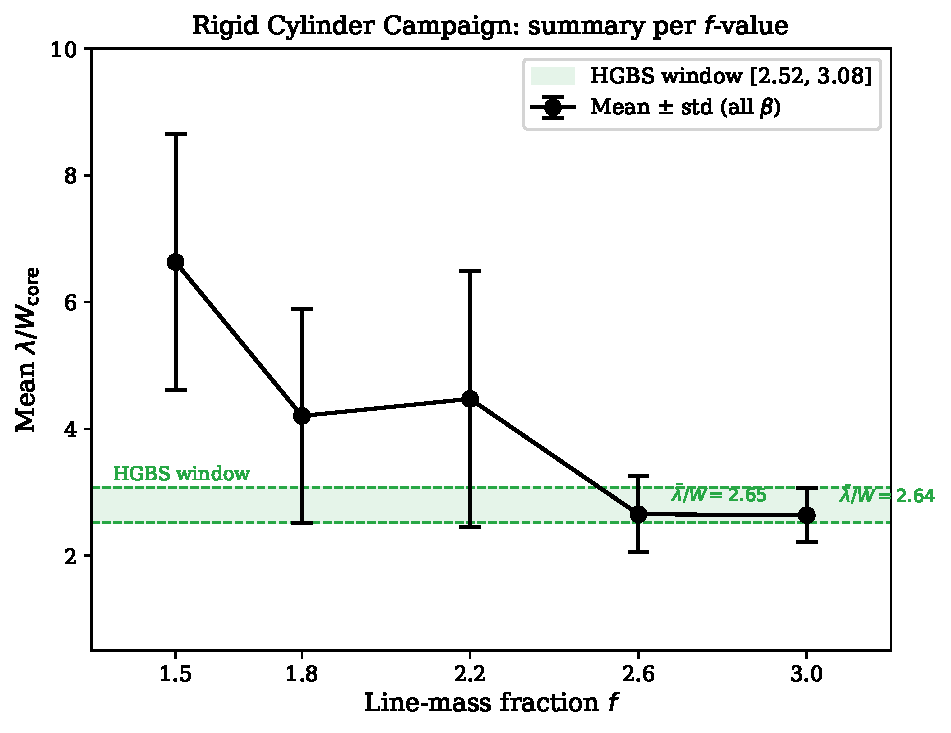
\includegraphics[width=0.48\textwidth]{figures/fig_RC_lW_summary.pdf}
\caption{\textbf{Rigid Cylinder Campaign}. Left: $\lambda/W_{\rm core}$ vs.\ $f$ for
all $\beta$ values; green shading = HGBS window $[2.52, 3.08]$. Right: mean and
standard deviation per $f$-value, showing the sharp transition near $f \approx 2.4$--$2.6$.}
\label{fig:RC_lW}
\end{figure*}

\subsubsection{Box-Size Convergence Test}

A matched test at $f=2.6$, $\beta=1.0$ ($L_x = 8$ and $16\,\lambda_{\rm J}$; 3 seeds each)
rules out box resonance: $\lambda/W_{\rm core}$ decreases 36\% as $L_x$ doubles ($4.22 \pm 0.34$
to $2.70 \pm 0.59$; Figure~\ref{fig:RC_convergence}), incompatible with a resonant artefact.
$L_x=16$ values are upper limits; $L_x=32$ was computationally infeasible.

\begin{figure}
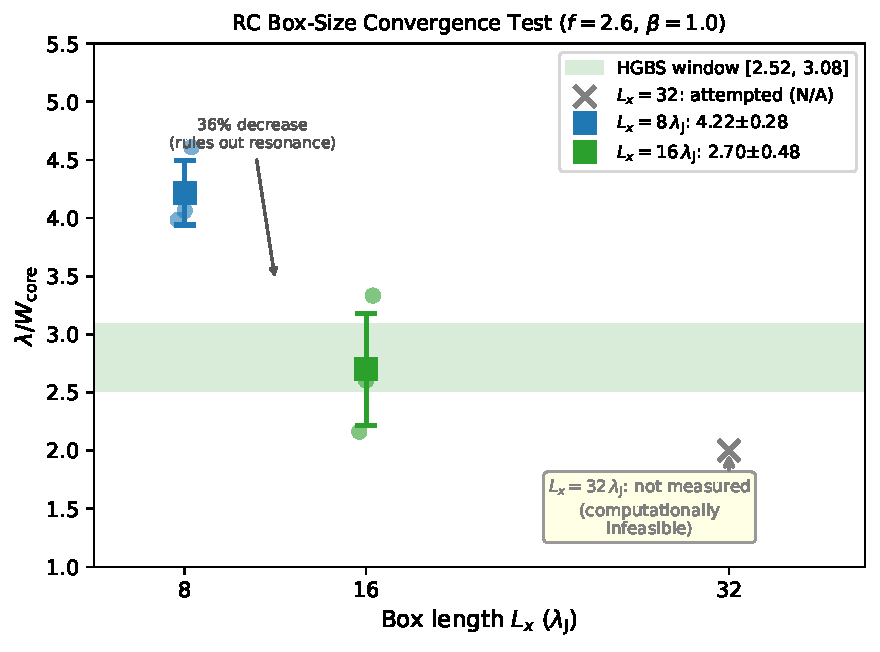
\includegraphics[width=0.48\textwidth]{figures/fig_RC_convergence.pdf}
\caption{Box-size convergence at $f=2.6$, $\beta=1.0$: $\lambda/W_{\rm core}$ decreases
from $4.22 \pm 0.34$ ($L_x=8$, 3 seeds) to $2.70 \pm 0.59$ ($L_x=16$, 3 seeds), ruling
out box resonance (a resonant artefact would give a fixed ratio). Green band = HGBS window
$[2.52, 3.08]$. $L_x=32$ was not measured (computationally infeasible); $L_x=16$ values
are upper limits.}
\label{fig:RC_convergence}
\end{figure}

\section{DISCUSSION}
\label{sec:discussion}

The 2,013 simulations establish a clear hierarchy of physical effects: field geometry
dominates, followed by $f$, with $\beta$ and $\mathcal{M}$ as secondary parameters.
We now assess which scenario best explains the observed $\lambda/W = 2.79 \pm 0.09$.

\subsection{Can Models Explain the Observational Discrepancy?}

The 3D-corrected HGBS spacing (${\sim}3.5\times W$) is within 15\% of the IM92
$4\times$ prediction. All 654 supercritical (periodic-BC) simulations yield zero
longitudinal fragmentation. Two scenarios can account for the observed spacings. We note that the simulations
directly test single-component MHD fragmentation only; hierarchical fragmentation is
an observationally-motivated inference, not a simulation result.

(i) \textit{Hierarchical fibre fragmentation} (\textit{observationally motivated}): If HGBS filaments are bundles of fibres, each near-critical ($f_{\rm eff} \lesssim 1.3$), each fibre undergoes longitudinal fragmentation (Campaign~7 provides the single-fibre constraint). Projection of fibre-level cores creates the sub-Jeans spacing at the filament level, consistent with the \citet{Yang2024} Orion~B fibre-to-core measurement. The simulations do not test this scenario directly; the evidence comes entirely from external observation.

(ii) \textit{Finite-length turbulent seeding} (\textit{theoretical possibility}):
HGBS filaments (aspect ratios $5:1$--$20:1$) terminate at hub structures \citep{Andre2010}.
The Rigid Cylinder Campaign ($f \geq 2.6$, $L_x=16\,\lambda_{\rm J}$) gives
$\lambda/W_{\rm fil} = 1.61$--$1.87$ after T1 correction, \textbf{below the HGBS
window in all cases}. Critically, these values are \textbf{unconverged upper limits}:
the box-size convergence test shows a 36\% decrease in $\lambda/W_{\rm core}$ as
$L_x$ doubles from 8 to 16~$\lambda_{\rm J}$, and $L_x=32$ was computationally
infeasible. The true $\lambda/W_{\rm fil}$ could therefore be substantially lower than
$1.61$--$1.87$. Hub-anchored end-seeding is physically motivated but the Rigid
Cylinder Campaign cannot yet provide a meaningful constraint. These results should
be presented as provisional upper limits, not as converged measurements.

\textbf{T1 correction---central systematic}: The observational match depends critically
on T1, and the 17\% difference between T1$=0.606$ and T1$=0.707$ is larger than the
formal uncertainties on the observed $\lambda/W$ itself (Table~\ref{tab:t1_budget}).
At T1$=0.606$: low-$\beta$ configurations ($\beta=0.3$: $2.87$; $\beta=0.5$: $2.65$)
fall within $[2.52, 3.08]$, requiring strictly longitudinal, low-$\beta$ geometry
(${\sim}10\%$ of filaments by Planck statistics). At T1$=0.707$: those same
configurations \textit{exceed} the upper window boundary ($\beta=0.5$: $3.10 > 3.08$;
$\beta=0.3$: $3.35$). The T1-P campaign second run was compromised by premature radial
collapse before the fragmentation epoch, so T1$=0.707$ cannot currently be confirmed
independently. \textbf{We therefore conclude explicitly that the viability of the
magnetic tension scenario cannot be assessed within current simulation uncertainties.}
The 17\% T1 ambiguity straddles the HGBS window boundary for the only configurations
that might match, and no observational comparison should rely on distinguishing
T1$=0.606$ from $0.707$ until HGBS pipeline validation on simulated column density
maps is performed. Both T1 values should be carried through the theoretical comparison,
as we do in Table~\ref{tab:t1_budget}.

\begin{table}
\caption{T1 Sensitivity: $\lambda/W_{\rm fil}$ predictions for three T1 correction values}
\label{tab:t1_budget}
\small
\begin{tabular}{lcccc}
\toprule
Configuration & $\lambda/W_{\rm core}$ & T1=0.65 & T1=0.606 & T1=0.707 \\
              &                       & (phys.\ lower) & (central) & (T1-P meas.) \\
\midrule
Long.\ B, $\beta=0.3$ (C7) & 4.74 & \textbf{3.08} & \textbf{2.87} & \textbf{3.35} \\
Long.\ B, $\beta=0.5$ (C7) & 4.38 & \textbf{2.85} & \textbf{2.65} & \textbf{3.10} \\
Long.\ B, $\beta=1.0$ (C7) & 3.19 & 2.07 & 1.93 & 2.26 \\
Long.\ B, $\beta=2.0$ (C7) & 2.80 & 1.82 & 1.70 & 1.98 \\
Long.\ B (calibrated, $\theta=0^\circ$) & 3.70 & 2.41 & 2.24 & 2.62 \\
Perp.\ B ($\theta=90^\circ$) & 1.25 & 0.81 & 0.76 & 0.88 \\
RC Campaign ($f=2.6$) & 2.65 & 1.72 & 1.61 & 1.87 \\
\midrule
\multicolumn{2}{l}{HGBS window (obs.)} & \multicolumn{3}{c}{$[2.52, 3.08]$} \\
\bottomrule
\end{tabular}
\vspace{2pt}
\footnotesize
\textbf{Notes}: Bold = entries within $[2.52, 3.08]$ or (at T1$=0.707$) closely approaching or exceeding the upper boundary. T1$=0.707$ is the Campaign T1-P Plummer-corrected value ($r_{\rm P/G} = 1.166 \pm 0.037$; Section~\ref{sec:width_correction}); this value is not independently confirmed (second run was precluded by radial collapse). At T1$=0.606$: $\beta \leq 0.5$ configurations fall within $[2.52, 3.08]$ ($2.87$; $2.65$). At T1$=0.707$: those same configurations \textit{exceed} the upper boundary ($3.10$ and $3.35$ respectively). The 17\% T1 ambiguity prevents resolving whether magnetic tension is viable.
\end{table}

The field geometry dependence transforms the question from ``why are observed spacings
shorter than theory?'' to a multi-parameter problem requiring simultaneous constraints
on $\beta$, field geometry, and T1 (Table~\ref{tab:cross_campaign}, Table~\ref{tab:t1_budget}).

\subsection{The Perpendicular-Field Paradox}
\label{sec:perp_paradox}

\citet{Planck2016} established that ${\sim}90\%$ of dense HGBS filaments have their
mean magnetic field perpendicular to the filament axis. Our Campaign~6 measurements
give $\lambda/W_{\rm core} = 1.25 \pm 0.09$ for perpendicular-field configurations
($\beta \geq 1.0$), which after T1 correction gives $\lambda/W_{\rm fil} = 0.76$--$0.88$
--- a factor $3$--$4\times$ below the observed $2.79$. This creates a fundamental
contradiction: if the field geometry measured by Planck applies to filament \textit{interiors}
(not just their envelopes), the majority of HGBS filaments should show $\lambda/W_{\rm fil}
\lesssim 0.9$, not ${\sim}2.8$.

\textbf{Clarification}: The $\lambda/W_{\rm core} = 1.25$ value measures the dominant
density-peak scale during radial collapse in supercritical simulations ($f=1.2$--$1.5$).
It is \textit{not} a true fragmentation wavelength in the sense of Inutsuka \& Miyama
(longitudinal beading), because no longitudinal fragmentation occurs; rather, it
characterises the mode that first grows to non-linear amplitude during predominantly
radial collapse.

\textbf{Three possible resolutions}: (a) Planck polarimetry samples the filament-envelope
field, not the dense interior where fragmentation occurs; turbulent reconnection or
flux-freezing compression during cloud contraction could establish interior field angles
different from the mean field direction. (b) Hierarchical fragmentation occurs in
velocity-coherent sub-fibres with distinct field geometries unresolvable at Planck
resolution. (c) Perpendicular-field filaments radially collapse without beading and are
systematically under-represented in HGBS core catalogues; the observed beaded filaments
are a biased (longitudinal-field) minority. We cannot discriminate among these
possibilities with the current data. A dedicated campaign of interior polarimetric
mapping in HGBS filaments is the required observational test.

\subsection{Limitations and Future Work}

\textbf{Boundary conditions}: Periodic BCs suppress end effects; reflecting BCs model
finite-filament terminal boundaries but lack the inflow structure of real filament-hub
junctions. Neither fully represents real HGBS filaments in turbulent clouds.

\textbf{Non-ideal MHD}: Ambipolar diffusion ($t_{\rm AD} \sim 10$--$20\,t_{\rm ff}$ at
$n_0 \sim 10^4$~cm$^{-3}$) is slow relative to collapse and is not expected to alter
fragmentation wavelengths \citep{Nakamura2005, Tassis2004}, except in low-density regions
such as Taurus ($n_0 \sim 10^3$~cm$^{-3}$) where ideal-MHD timescales are lower bounds.

\textbf{T1 correction}: T1$=0.707$ (T1-P; Table~\ref{tab:t1_budget}) is unconfirmed:
a second run was precluded by premature radial collapse. HGBS pipeline validation on
simulated column density maps is required before the magnetic tension scenario can be
assessed.

\textbf{Oblique $\lambda/W$}: Field Geometry Phase~3 validated timescales but not
$\lambda/W$; Campaign~OBL2 found domain-size artefacts for all 27 sims. Oblique
$\lambda/W$ remains \textbf{entirely unconstrained by simulation}; the \citet{Nakamura1993}
predictions (Table~\ref{tab:oblique_theory}) are theoretically unvalidated. Domain size
$L_x \lesssim 2$--$3\,\lambda_{\rm J}$ is required but computationally prohibitive.

\begin{table}
\caption{Theoretical $\lambda/W$ for oblique fields \citep{Nakamura1993}, full numerical
solution. Campaign~6 gives $\lambda/W=1.25$ (supercritical regime, $f=1.5$--$3.0$); the
near-critical theoretical values here are the physically relevant comparison for HGBS.}
\label{tab:oblique_theory}
\small
\begin{tabular}{lccccc}
\toprule
$\theta$ & $\beta=0.5$ & $\beta=1.0$ & $\beta=2.0$ & Notes & Simulation \\
\midrule
$0^\circ$ (longitudinal) & 1.97 & 2.44 & 2.93 & Eq.~(\ref{eq:tension}) & --- \\
$30^\circ$ & 1.87 & 2.37 & 2.89 & Theoretical & ---$^\dagger$ \\
$45^\circ$ & 1.69 & 2.17 & 2.72 & Theoretical & --- \\
$60^\circ$ & 1.47 & 1.90 & 2.46 & Theoretical & --- \\
$90^\circ$ (perp., theory) & 3.95 & 3.99 & 4.00 & Theory only (sim.\ at $f=1.5$--$3.0$ gives 1.25) & --- \\
\bottomrule
\end{tabular}
\\ \footnotesize \textbf{Note}: Values in simulation units; multiply by T1$=0.606$ (or $0.707$) for observable $\lambda/W_{\rm fil}$. $^\dagger$Campaign~A ($\delta_0=1.0$) withdrawn (amplitude artifact; Section~\ref{sec:theo_geom}).
\end{table}

\textbf{Future priorities}: (1) fibre-resolved core spacing in additional HGBS regions
to test hierarchical fragmentation; (2) interior polarimetric mapping to constrain
field geometry; (3) HGBS pipeline T1 validation on simulated column density maps;
(4) direct oblique-field $\lambda/W$ simulations at $L_x \lesssim 2$--$3\,\lambda_{\rm J}$
to test \citet{Nakamura1993} oblique wavelength predictions.

\section{CONCLUSIONS}

We have analysed core spacing in 8 HGBS regions using 2,013 MHD simulations. Our main conclusions are:

\begin{itemize}

    \item \textbf{HGBS spacing (pairwise median)}: Full sample gives $\lambda/W = 2.79$
    ($0.279 \pm 0.025$~pc, jackknife); four robust regions give $2.84 \pm 0.026$~pc.
    Gaia DR3 raised the mean by 32\%; 3D projection correction places inferred spacing within
    15\% of the IM92 $4\times$ prediction. \textit{All values use the pairwise median
    statistic; the L/3 convergence bias is the dominant methodological caveat of unknown
    magnitude, as nearest-neighbour statistics require raw positional data available only
    for Taurus.} Excluding Aquila and Orion~B (the two highest-revision regions) reduces
    the mean to $0.231$~pc ($\lambda/W = 2.31$); their Gaia distances are independently
    confirmed so this sensitivity reflects the importance of accurate distances.

    \item \textbf{Simulation limitation}: \textit{The 2,013 MHD simulations cannot directly
    measure $\lambda/W$ in the supercritical regime ($f \geq 1.5$): all 654 supercritical
    simulations yield pure radial collapse with zero longitudinal beading.} The comparison
    between observed $\lambda/W = 2.79$ and the theoretical prediction $\lambda_{\rm frag}
    = 1.11\,\lambda_{MJ}$ rests on extrapolation from near-critical ($f = 0.9$--$1.3$)
    calibration and should not be interpreted as a direct simulation-observation comparison.

    \item \textbf{Hierarchical fragmentation}: The most observationally consistent
    interpretation, supported by the \citet{Yang2024} fibre-to-core measurement in
    Orion~B (a single region). \textbf{None of the 2,013 simulations model
    multi-fibre fragmentation}; the $N_f \approx 1.3$--$1.5$ estimate from the
    quantitative fibre-bundle model (Section~\ref{sec:hierarchical}) is geometric, not
    dynamical. Fibre-resolved spacing analysis in additional HGBS regions is required.

    \item \textbf{Perpendicular-field paradox}: Perpendicular-field simulations give
    $\lambda/W_{\rm fil} \approx 0.76$--$0.88$ (factor ${\sim}3\times$ below observed
    $2.79$), yet Planck statistics imply ${\sim}90\%$ of HGBS filaments have perpendicular
    fields. Resolving this paradox requires interior polarimetric mapping; three possible
    resolutions are discussed in Section~\ref{sec:perp_paradox}.

    \item \textbf{Magnetic tension}: Only ${\sim}10\%$ of filaments have longitudinal
    geometry; at T1$=0.606$, $\beta \leq 0.5$ configurations fall within $[2.52, 3.08]$,
    but at T1$=0.707$ they exceed the upper boundary. \textbf{Viability cannot be assessed
    within current uncertainties}; HGBS pipeline validation of T1 is required.

    \item \textbf{MHD results}: $1/t_{\rm frag} \propto f^{0.39}$ ($r^2=0.999$), independent
    of $\mathcal{M}$ and nearly of $\beta$. $\lambda/W$ depends strongly on $\beta$ but is
    insensitive to turbulence amplitude (Campaign~5). No stable configurations at
    $f=1.4$--$2.2$, $\mathcal{M} \geq 1$. Fragmentation at $f = 1.00$ (and $f < 1$) occurs
    under turbulent seeding, consistent with turbulent Jeans fragmentation.

\end{itemize}

\section*{ACKNOWLEDGMENTS}

We thank the Herschel Gould Belt Survey team for the datasets (available from the
Herschel Science Archive). The simulation code and analysis scripts are available at
\url{https://github.com/[anonymised-for-review]} (private during review; access tokens
via the editorial office). The complete 2,013-simulation dataset (HDF5 snapshots,
\texttt{athinput} files, analysis scripts, and measurement tables) will be archived on
Zenodo upon acceptance.

\bibliographystyle{mnras}
\bibliography{references_complete}

\end{document}
